% A LaTeX template for MSc Thesis submissions to 
% Politecnico di Milano (PoliMi) - School of Industrial and Information Engineering
%
% S. Bonetti, A. Gruttadauria, G. Mescolini, A. Zingaro
% e-mail: template-tesi-ingind@polimi.it
%
% Last Revision: October 2021
%
% Copyright 2021 Politecnico di Milano, Italy. NC-BY

\documentclass{Configuration_Files/PoliMi3i_thesis}

%------------------------------------------------------------------------------
%	REQUIRED PACKAGES AND  CONFIGURATIONS
%------------------------------------------------------------------------------

% CONFIGURATIONS
\usepackage{parskip} % For paragraph layout
\usepackage{setspace} % For using single or double spacing
\usepackage{emptypage} % To insert empty pages
\usepackage{multicol} % To write in multiple columns (executive summary)
\setlength\columnsep{15pt} % Column separation in executive summary
\setlength\parindent{0pt} % Indentation
\raggedbottom  

% PACKAGES FOR TITLES
\usepackage{titlesec}
% \titlespacing{\section}{left spacing}{before spacing}{after spacing}
\titlespacing{\section}{0pt}{3.3ex}{2ex}
\titlespacing{\subsection}{0pt}{3.3ex}{1.65ex}
\titlespacing{\subsubsection}{0pt}{3.3ex}{1ex}
\usepackage{color}

% PACKAGES FOR LANGUAGE AND FONT
\usepackage[english]{babel} % The document is in English  
\usepackage[utf8]{inputenc} % UTF8 encoding
\usepackage[T1]{fontenc} % Font encoding
\usepackage[11pt]{moresize} % Big fonts

% PACKAGES FOR IMAGES
\usepackage{graphicx}
\usepackage{transparent} % Enables transparent images
\usepackage{eso-pic} % For the background picture on the title page
\usepackage{subfig} % Numbered and caption subfigures using \subfloat.
\usepackage{tikz} % A package for high-quality hand-made figures.
\usetikzlibrary{}
\graphicspath{{./Images/}} % Directory of the images
\usepackage{caption} % Coloured captions
\usepackage{xcolor} % Coloured captions
\usepackage{amsthm,thmtools,xcolor} % Coloured "Theorem"
\usepackage{float}

% STANDARD MATH PACKAGES
\usepackage{amsmath}
\usepackage{amsthm}
\usepackage{amssymb}
\usepackage{amsfonts}
\usepackage{bm}
\usepackage[overload]{empheq} % For braced-style systems of equations.
\usepackage{fix-cm} % To override original LaTeX restrictions on sizes

% PACKAGES FOR TABLES
\usepackage{tabularx}
\usepackage{longtable} % Tables that can span several pages
\usepackage{colortbl}

% PACKAGES FOR ALGORITHMS (PSEUDO-CODE)
\usepackage{algorithm}
\usepackage{algorithmic}

% PACKAGES FOR REFERENCES & BIBLIOGRAPHY
\usepackage[colorlinks=true,linkcolor=black,anchorcolor=black,citecolor=black,filecolor=black,menucolor=black,runcolor=black,urlcolor=black]{hyperref} % Adds clickable links at references
\usepackage{cleveref}
\usepackage[square, numbers, sort&compress]{natbib} % Square brackets, citing references with numbers, citations sorted by appearance in the text and compressed
\bibliographystyle{abbrvnat} % You may use a different style adapted to your field

% OTHER PACKAGES
\usepackage{pdfpages} % To include a pdf file
\usepackage{afterpage}
\usepackage{lipsum} % DUMMY PACKAGE
\usepackage{fancyhdr} % For the headers
\fancyhf{}

% Input of configuration file. Do not change config.tex file unless you really know what you are doing. 
\input{Configuration_Files/config}

%----------------------------------------------------------------------------
%	NEW COMMANDS DEFINED
%----------------------------------------------------------------------------

% EXAMPLES OF NEW COMMANDS
\newcommand{\bea}{\begin{eqnarray}} % Shortcut for equation arrays
\newcommand{\eea}{\end{eqnarray}}
\newcommand{\e}[1]{\times 10^{#1}}  % Powers of 10 notation

%----------------------------------------------------------------------------
%	ADD YOUR PACKAGES (be careful of package interaction)
%----------------------------------------------------------------------------

%----------------------------------------------------------------------------
%	ADD YOUR DEFINITIONS AND COMMANDS (be careful of existing commands)
%----------------------------------------------------------------------------

%----------------------------------------------------------------------------
%	BEGIN OF YOUR DOCUMENT
%----------------------------------------------------------------------------

\begin{document}

\fancypagestyle{plain}{%
	\fancyhf{} % Clear all header and footer fields
	\fancyhead[RO,RE]{\thepage} %RO=right odd, RE=right even
	\renewcommand{\headrulewidth}{0pt}
	\renewcommand{\footrulewidth}{0pt}}

%----------------------------------------------------------------------------
%	TITLE PAGE
%----------------------------------------------------------------------------

\pagestyle{empty} % No page numbers
\frontmatter % Use roman page numbering style (i, ii, iii, iv...) for the preamble pages

\puttitle{
	title=Systems and Methods for Big and Unstructured Data Project,
	name1=Cristiano Battistini, % Author Name and Surname
	name2=Carlo Cardignan 11001182,
	name3=,
	name4=,
	name5=,
	academicyear=2023-2024,
	groupnumber=GroupNumber
} % These info will be put into your Title page 

%----------------------------------------------------------------------------
%	PREAMBLE PAGES: ABSTRACT (inglese e italiano), EXECUTIVE SUMMARY
%----------------------------------------------------------------------------
\startpreamble
\setcounter{page}{1} % Set page counter to 1

%----------------------------------------------------------------------------
%	LIST OF CONTENTS/FIGURES/TABLES/SYMBOLS
%----------------------------------------------------------------------------

% TABLE OF CONTENTS
\thispagestyle{empty}
\tableofcontents % Table of contents 
\thispagestyle{empty}
\cleardoublepage

%-------------------------------------------------------------------------
%	THESIS MAIN TEXT
%-------------------------------------------------------------------------
% In the main text of your thesis you can write the chapters in two different ways:
%
%(1) As presented in this template you can write:
%    \chapter{Title of the chapter}
%    *body of the chapter*
%
%(2) You can write your chapter in a separated .tex file and then include it in the main file with the following command:
%    \chapter{Title of the chapter}
%    \input{chapter_file.tex}
%
% Especially for long thesis, we recommend you the second option.

\addtocontents{toc}{\vspace{2em}} % Add a gap in the Contents, for aesthetics
\mainmatter % Begin numeric (1,2,3...) page numbering

\chapter{Introduction}
\label{ch:chapter_one}%
% The \label{...}% enables to remove the small indentation that is generated, always leave the % symbol.

\section{Introduction}
\label{sec:section_Introduction}
The advent of data-driven strategies in soccer has revolutionized the sport, providing insights that drive decisions, from player selection to game tactics. There are indeed many examples of clubs that have scouted top talent by leveraging data analysis. What's more, the millions of fans of the sport love to follow the statistics, to see the analytics of their idols in smartphone apps.\\
Our project builds on this data-centric approach, leveraging a detailed data set that encapsulates the multifaceted nature of soccer, including player statistics, club data, and competition history. We chose MongoDB because its non-relational structure is particularly well suited to handle the diversity and volume of data we are dealing with. Unlike traditional relational databases, MongoDB's flexible data model allows us to store and process different types of data without the need for a predefined schema.\\
MongoDB, being a document-oriented database, allows each player, club or competition to be represented as a document with a rich and dynamic set of attributes. In addition, MongoDB's horizontal scalability through automatic sharding is critical for handling large volumes of data, such as those generated in modern soccer. The performance of this technology is in fact optimal even as the data size increases. \\
All of this allows us to dynamically adapt to the evolving nature of the dataset, reflecting the real-world fluidity of soccer team compositions and league structures, keeping in mind that nowadays there is always a competition game to watch.\\
Our goal is to extract meaningful patterns and insights that can influence various factors, such as talent scouting but also match analysis. The dataset includes detailed details on players, with their appearances and ratings, club situations, and the competitive landscape of the major leagues.

\chapter{Data Wrangling/Data Generation}
\label{ch:chapter_two}%
% The \label{...}% enables to remove the small indentation that is generated, always leave the % symbol.

\section{Chapter Introduction}
\label{sec:section_Data_Wrangling/Data_Generation}
A cleanup and standardization of football-related data was necessary. This process included replacing long, detailed descriptive strings with one- or two-character abbreviations to make the data more manageable and optimize the size of the database. The operation was done manually using the "find and replace" function of the Visual Studio Code software. Specifically, the "description" attribute within the "game\_events"  dataset was simplified by removing unnecessary details such as the total number of season goals or the specification of tournament goals, keeping only the essentials such as the type of shot that led to the goal. This process made the data more streamlined and focused on relevant aspects for later analysis. The following tables describe what was changed in the initial datasets.
\newpage
\subsection{Players}
\begin{table}[ht]
	\centering
	\begin{tabular}{|l|l|l|l|}
		\hline
		\textbf{Original Dataset} & \textbf{Attribute} & \textbf{Old Value} & \textbf{New Value} \\ \hline
		players                   & sub\_position      & Attacking Midfield & AM                 \\ \hline
		players                   & sub\_position      & Defensive Midfield & DM                 \\ \hline
		players                   & sub\_position      & Goalkeeper         & G                  \\ \hline
		players                   & sub\_position      & Centre-Forward     & CF                 \\ \hline
		players                   & sub\_position      & Centre-Back        & CB                 \\ \hline
		players                   & sub\_position      & Central Midfield   & CM                 \\ \hline
		players                   & sub\_position      & Left Winger        & LW                 \\ \hline
		players                   & sub\_position      & Right Winger       & RW                 \\ \hline
		players                   & sub\_position      & Right-Back         & RB                 \\ \hline
		players                   & sub\_position      & Left-Back          & LB                 \\ \hline
		players                   & sub\_position      & Left Midfield      & LM                 \\ \hline
		players                   & sub\_position      & Right Midfield     & RM                 \\ \hline
		players                   & sub\_position      & Second Striker     & ST                 \\ \hline
		players                   & position           & Defender           & D                  \\ \hline
		players                   & position           & Midfield           & C                  \\ \hline
		players                   & position           & Attack             & A                  \\ \hline
		players                   & position           & Missing            & M                  \\ \hline
		players                   & position           & GoalKeeper         & G                  \\ \hline
		players                   & foot               & right              & R                  \\ \hline
		players                   & foot               & left               & L                  \\ \hline
	\end{tabular}
	\caption{Your caption here}
	\label{your-label-here}
\end{table}
\newpage
\subsection{Game events}
\begin{table}[ht]
	\centering
	\begin{tabular}{|l|l|l|l|}
		\hline
		\textbf{Original Dataset} & \textbf{Attribute} & \textbf{Old Value}     & \textbf{New Value} \\ \hline
		game\_events              & description        & Right-footed shot      & R                  \\ \hline
		game\_events              & description        & Penalty                & P                  \\ \hline
		game\_events              & description        & Direct free kick       & F                  \\ \hline
		game\_events              & description        & Left-footed shot       & L                  \\ \hline
		game\_events              & description        & Header                 & H                  \\ \hline
		game\_events              & description        & Tap-in                 & T                  \\ \hline
		game\_events              & description        & Deflected shot on goal & D                  \\ \hline
		game\_events              & description        & Long distance kick     & K                  \\ \hline
		game\_events              & description        & Own goal               & O                  \\ \hline
		game\_events              & description        & Solo run               & S                  \\ \hline
		game\_events              & description        & Counter attack goal    & C                  \\ \hline
		game\_events              & description        & Chest                  & Q                  \\ \hline
		game\_events              & description        & Penalty rebound        & B                  \\ \hline
		game\_events              & description        & Direct corner          & N                  \\ \hline
	\end{tabular}
	\caption{Your caption here}
	\label{your-label-here}
\end{table}
\subsection{club games}
\begin{table}[ht]
	\centering
	\begin{tabular}{|l|l|l|l|}
		\hline
		\textbf{Original Dataset} & \textbf{Attribute} & \textbf{Old Value} & \textbf{New Value} \\ \hline
		club\_games               & hosting            & Home               & H                  \\ \hline
		club\_games               & hosting            & Away               & A                  \\ \hline
	\end{tabular}
	\caption{Your caption here}
	\label{your-label-here}
\end{table}
\section{Original Data}
Initially, the data were distributed in several datasets: 'clubs', 'club\_games', 'competitions', 'games', 'game\_events', 'player', 'player\_valuations' and 'appearances'. To optimize organization and accessibility, a restructuring into three main collections in the 'football' database was adopted. These are the initial datasets and their attributes:
\begin{tabular}{|l|p{13cm}|}
	\hline
	\textbf{Dataset name} & \textbf{Attributes}                       \\
	\hline
	players
	                      & player\_id,                               \\
	                      & first\_name,                              \\
	                      & last\_name,                               \\
	                      & name,                                     \\
	                      & last\_season,                             \\
	                      & current\_club\_id,                        \\
	                      & player\_code,                             \\
	                      & country\_of\_birth,                       \\
	                      & city\_of\_birth,                          \\
	                      & country\_of\_citizenship,                 \\
	                      & date\_of\_birth,                          \\
	                      & sub\_position,                            \\
	                      & position,                                 \\
	                      & foot,                                     \\
	                      & height\_in\_cm,                           \\
	                      & market\_value\_in\_eur,                   \\
	                      & highest\_market\_value\_in\_eur,          \\
	                      & contract\_expiration\_date,               \\
	                      & agent\_name,                              \\
	                      & image\_url,                               \\
	                      & url,                                      \\
	                      & current\_club\_domestic\_competition\_id, \\
	                      & current\_club\_name                       \\
	\hline
	player\_valuations
	                      & player\_id,                               \\
	                      & last\_season,                             \\
	                      & datetime,                                 \\
	                      & date,                                     \\
	                      & dateweek,                                 \\
	                      & market\_value\_in\_eur,                   \\
	                      & n,                                        \\
	                      & current\_club\_id,                        \\
	                      & player\_club\_domestic\_competition\_id   \\
	\hline
	
\end{tabular}

\begin{tabular}{|l|p{13cm}|}
	\hline
	\textbf{Dataset name} & \textbf{Attributes}                       \\
	\hline
appearances
	                      & appearance\_id,                           \\
	                      & game\_id,                                 \\
	                      & player\_id,                               \\
	                      & player\_club\_id,                         \\
	                      & player\_current\_club\_id,                \\
	                      & date,                                     \\
	                      & player\_name,                             \\
	                      & competition\_id,                          \\
	                      & yellow\_cards,                            \\
	                      & red\_cards,                               \\
	                      & goals,                                    \\
	                      & assists,                                  \\
	                      & minutes\_played                           \\
	\hline
	competitions
	                      & competition\_id,                          \\
	                      & competition\_code,                        \\
	                      & name,                                     \\
	                      & sub\_type,                                \\
	                      & type,                                     \\
	                      & country\_id,                              \\
	                      & country\_name,                            \\
	                      & domestic\_league\_code,                   \\
	                      & confederation,                            \\
	                      & url,                                      \\
	                      & club\_games,                              \\
	                      & game\_id,                                 \\
	                      & club\_id,                                 \\
	                      & own\_goals,                               \\
	                      & own\_position,                            \\
	                      & own\_manager\_name,                       \\
	                      & opponent\_id,                             \\
	                      & opponent\_goals,                          \\
	                      & opponent\_position,                       \\
	                      & opponent\_manager\_name,                  \\
	                      & hosting,                                  \\
	                      & is\_win                                   \\
	\hline
\end{tabular}


\begin{tabular}{|l|p{13cm}|}
	\hline
	\textbf{Dataset name} & \textbf{Attributes}                       \\
	\hline
    games
    & game\_id,                                 \\
    & competition\_id,                          \\
    & season,                                   \\
    & round,                                    \\
    & date,                                     \\
    & home\_club\_id,                           \\
    & away\_club\_id,                           \\
    & home\_club\_goals,                        \\
    & away\_club\_goals,                        \\
    & home\_club\_position,                     \\
    & away\_club\_position,                     \\
    & home\_club\_manager\_name,                \\
    & away\_club\_manager\_name,                \\
    & stadium,                                  \\
    & attendance,                               \\
    & referee,                                  \\
    & url,                                      \\
    & home\_club\_name,                         \\
    & away\_club\_name,                         \\
    & aggregate,                                \\
    & competition\_type,                        \\
    & clubs,                                    \\
    & club\_id,                                 \\
    & club\_code,                               \\
    & name,                                     \\
    & domestic\_competition\_id,                \\
    & total\_market\_value,                     \\
    & squad\_size,                              \\
    & average\_age,                             \\
    & foreigners\_number,                       \\
    & foreigners\_percentage,                   \\
    & national\_team\_players,                  \\
    & stadium\_name,                            \\
    & stadium\_seats,                           \\
    & net\_transfer\_record,                    \\
    & coach\_name,                              \\
    & last\_season,                             \\
    & url                                       \\
\hline
\end{tabular}

\begin{tabular}{|l|p{13cm}|}
	\hline
	\textbf{Dataset name} & \textbf{Attributes}                       \\
	\hline
    game\_events
    & game\_id,                                 \\
    & minute,                                   \\
    & type,                                     \\
    & club\_id,                                 \\
    & player\_id,                               \\
    & description,                              \\
    & player\_in\_id                            \\
\hline
\end{tabular}

The 'player' collection now integrates player information with related 'valuations' and 'appearances', thanks to the Python script 'players\_complete\_info.py'. The 'clubs' collection encapsulates within it the 'club\_games', which in turn contain details about 'game\_events', aggregated via the 'club\_and\_games.py' script. Finally, the 'competitions' collection was enriched with the associated 'games' and their respective 'game\_events' through the use of the 'competitions\_and\_games.py' script.
In merging multiple datasets, attributes that were repeated were removed both to save space and because they were unnecessary to the context outlined.
In the following repository \\
(at this URL \url{https://github.com/cristianobattistini/smbud}) it is possible to observe the python code for the updates to the original datasets.


\chapter{Dataset}
\label{ch:chapter_three}%

\section{Dataset}

Dataset
The selected dataset is a large collection of football data, derived primarily from Transfermarkt. Updated regularly, it offers accurate data on more than 60,000 global competition matches, details on 400 clubs, and statistics on more than 30,000 players, including current and historical market values, physical characteristics, team membership, and individual performances. More than 1.2 million records detail competitive performances, such as appearances and cards. It is possible to observe the original one, saved in \url{www.kaggle.com} , at this link:
\url{https://www.kaggle.com/datasets/thedevastator/football-data-competitions-clubs-players-statist }
After the Data Wrangling/Data Generation changes, the MongoDB database, called football, has the following collections and statistics:
\begin{itemize}
    \item 'clubs' collection: 411 documents, with an average size of 108.74 kB per document. Total size of indexes: 20.48 kB.
    \item 'Competitions' collection: 43 documents, with an average size of 974.35 kB per document. Total size of indexes: 20.48 kB.
    \item 'Players' collection: 28,459  documents, with an average size of 7.45 kB per document. Total size of indexes: 409.60 kB.
\end{itemize}
All the collections contain one or more arrays of sub-dcouments. Some sub-documents contain also other sub-documents.

\begin{figure}[htbp]
    \centering
    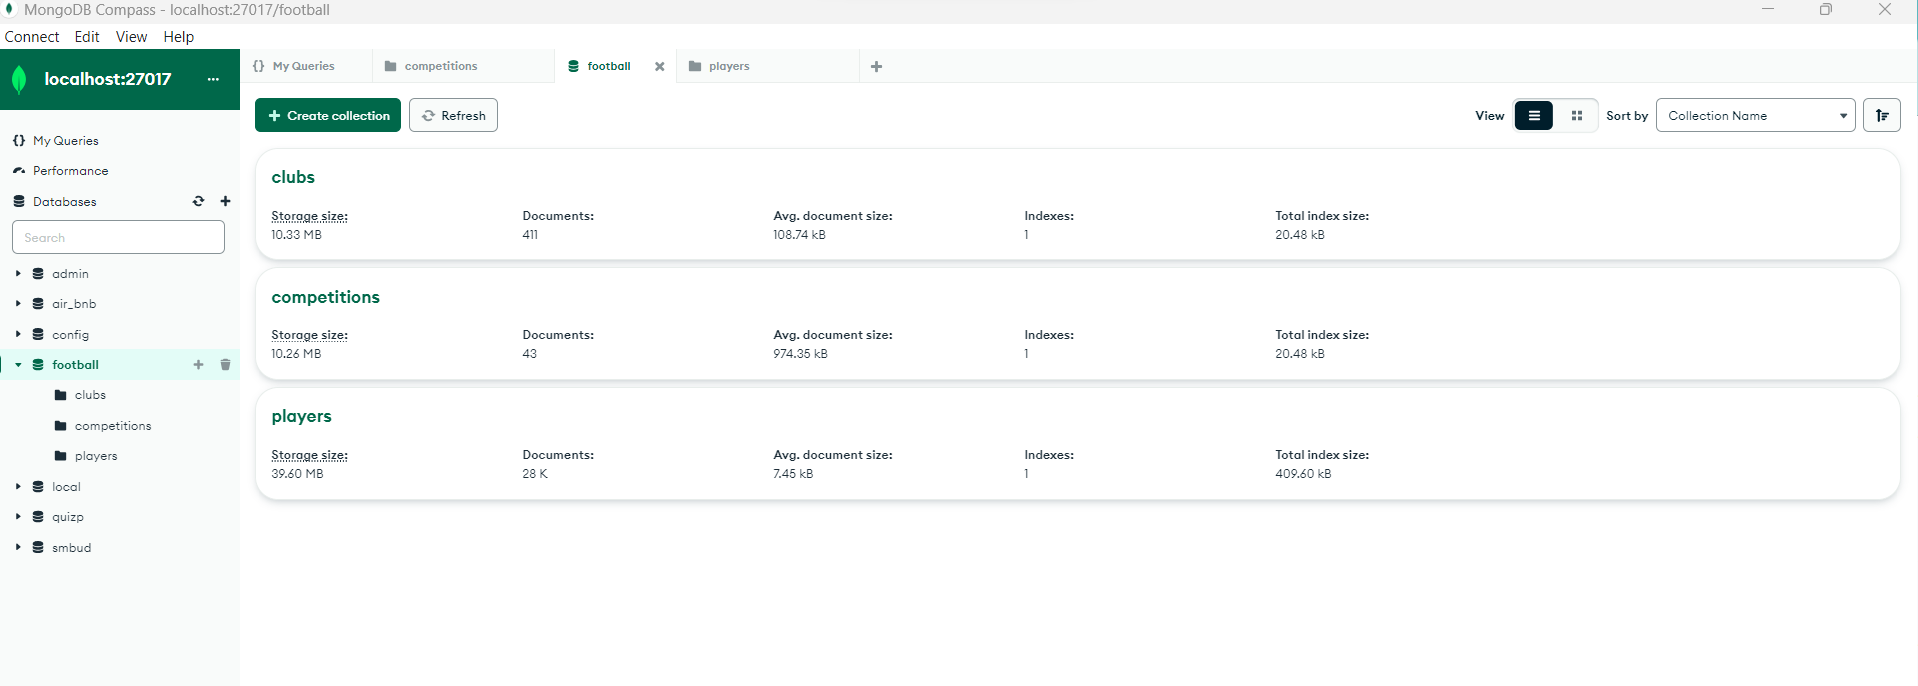
\includegraphics[scale=0.45]{Images/Dataset/football.png}
    \caption{Football Dataset}
\end{figure}
\newpage
\section{Collections}
\subsection{Clubs}
\begin{figure}[htbp]
    \centering
    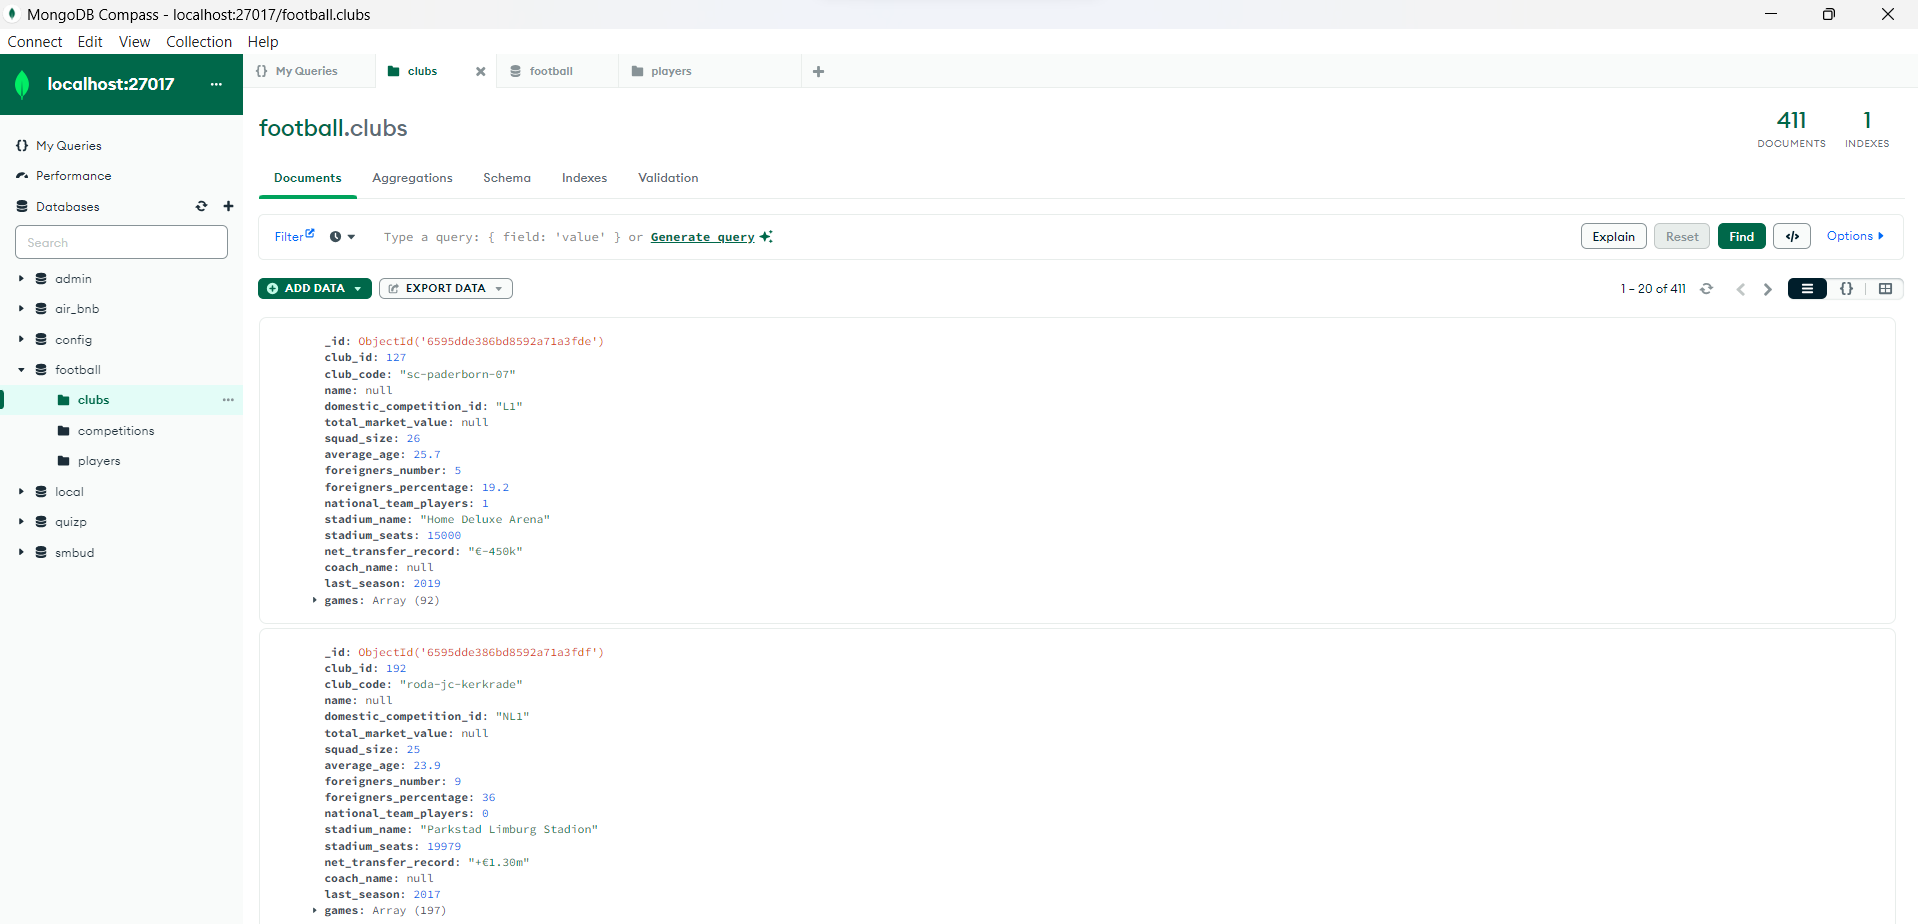
\includegraphics[scale=0.45]{Images/Dataset/clubs.png}
    \caption{Clubs Collection}
\end{figure}
    \begin{tabular}{|l|l|p{8cm}|}
    \hline
    \textbf{Attribute}              & \textbf{Type}           & \textbf{Description}                                                                 \\ \hline
    \_id                            & ObjectId                & A unique identifier for the document.                                                               \\ \hline
    club\_id                        & Int32                   & An integer representing the club's unique ID.                                                      \\ \hline
    club\_code                      & String                  & A textual code that uniquely identifies the club.                                                  \\ \hline
    name                            & String                  & The official name of the club.                                                                     \\ \hline
    domestic\_competition\_id       & String                  & The ID of the domestic league in which the club competes.                                           \\ \hline
    total\_market\_value            & Null                    & The total market value of the club, currently not available.                                        \\ \hline
    squad\_size                     & Int32                   & The number of players in the club's squad.                                                         \\ \hline
    average\_age                    & Double                  & The average age of the players in the squad.                                                       \\ \hline
    foreigners\_number              & Int32                   & The count of foreign players in the squad.                                                         \\ \hline
    foreigners\_percentage          & Double                  & The percentage of foreign players relative to the total squad size.                                \\ \hline
    national\_team\_players         & Int32                   & The number of players who are also national team members.                                          \\ \hline
    stadium\_name                   & String                  & The name of the club's home stadium.                                                               \\ \hline
    stadium\_seats                  & Int32                   & The seating capacity of the club's stadium.                                                        \\ \hline
    net\_transfer\_record           & Null                    & The net financial record of player transfers, currently not available.                             \\ \hline
    coach\_name                     & String                  & The name of the club's coach.                                                                      \\ \hline
    last\_season                    & Int32                   & The most recent season the club competed in.                                                       \\ \hline
    games                           & Array (of objects)      & A textual code that uniquely identifies the club.                                                  \\ \hline
    \end{tabular}
\subsubsection{Game Object inside Club}
    \begin{tabular}{|l|l|p{8cm}|}
    \hline
    \textbf{Attribute}            & \textbf{Type}           & \textbf{Description}                                                                                  \\ \hline
    game\_id                      & Int32                   & The unique identifier for the game.                                                                   \\ \hline
    own\_goals                    & Int32                   & The number of goals scored by the club.                                                               \\ \hline
    own\_position                 & Int32                   & The league position of the club at the time of the game.                                              \\ \hline
    own\_manager\_name            & String                  & The name of the club's manager.                                                                       \\ \hline
    opponent\_id                  & Int32                   & The unique identifier for the opponent club.                                                          \\ \hline
    opponent\_goals               & Int32                   & The number of goals scored by the opponent.                                                           \\ \hline
    opponent\_position            & Int32                   & The league position of the opponent at the time of the game.                                          \\ \hline
    opponent\_manager\_name       & String                  & The name of the opponent's manager.                                                                   \\ \hline
    hosting                       & String                  & A character indicating whether the club was hosting the game ('H' for home, ‘A’ for away).             \\ \hline
    is\_win                       & Int32                   & Indicates the outcome of the game (e.g., 0 for loss or draw, 1 for win).                              \\ \hline
    events                        & Array (of objects)      & A list of significant events during the game, with each event as an object containing its own set of attributes. \\ \hline
    \end{tabular}
\subsubsection{Events inside Games inside Clubs}
    \begin{tabular}{|l|l|p{8cm}|}
    \hline
    \textbf{Attribute}    & \textbf{Type}          & \textbf{Description}                                                                 \\ \hline
    minute                & Int32                  & The match time in minutes when the event occurred.                                   \\ \hline
    type                  & String                 & The category of the event, e.g., "Substitutions” or “Goals”                         \\ \hline
    player\_id            & Int32                  & The unique identifier of the player involved in the event.                          \\ \hline
    description           & Null/String            & A detailed description of the event, if available.                                  \\ \hline
    player\_in\_id        & Int32                  & The unique identifier of the player substituted into the game, relevant for substitution events. \\ \hline
    \end{tabular}
    


    \newpage
\subsection{Competition}
\begin{figure}[htbp]
    \centering
    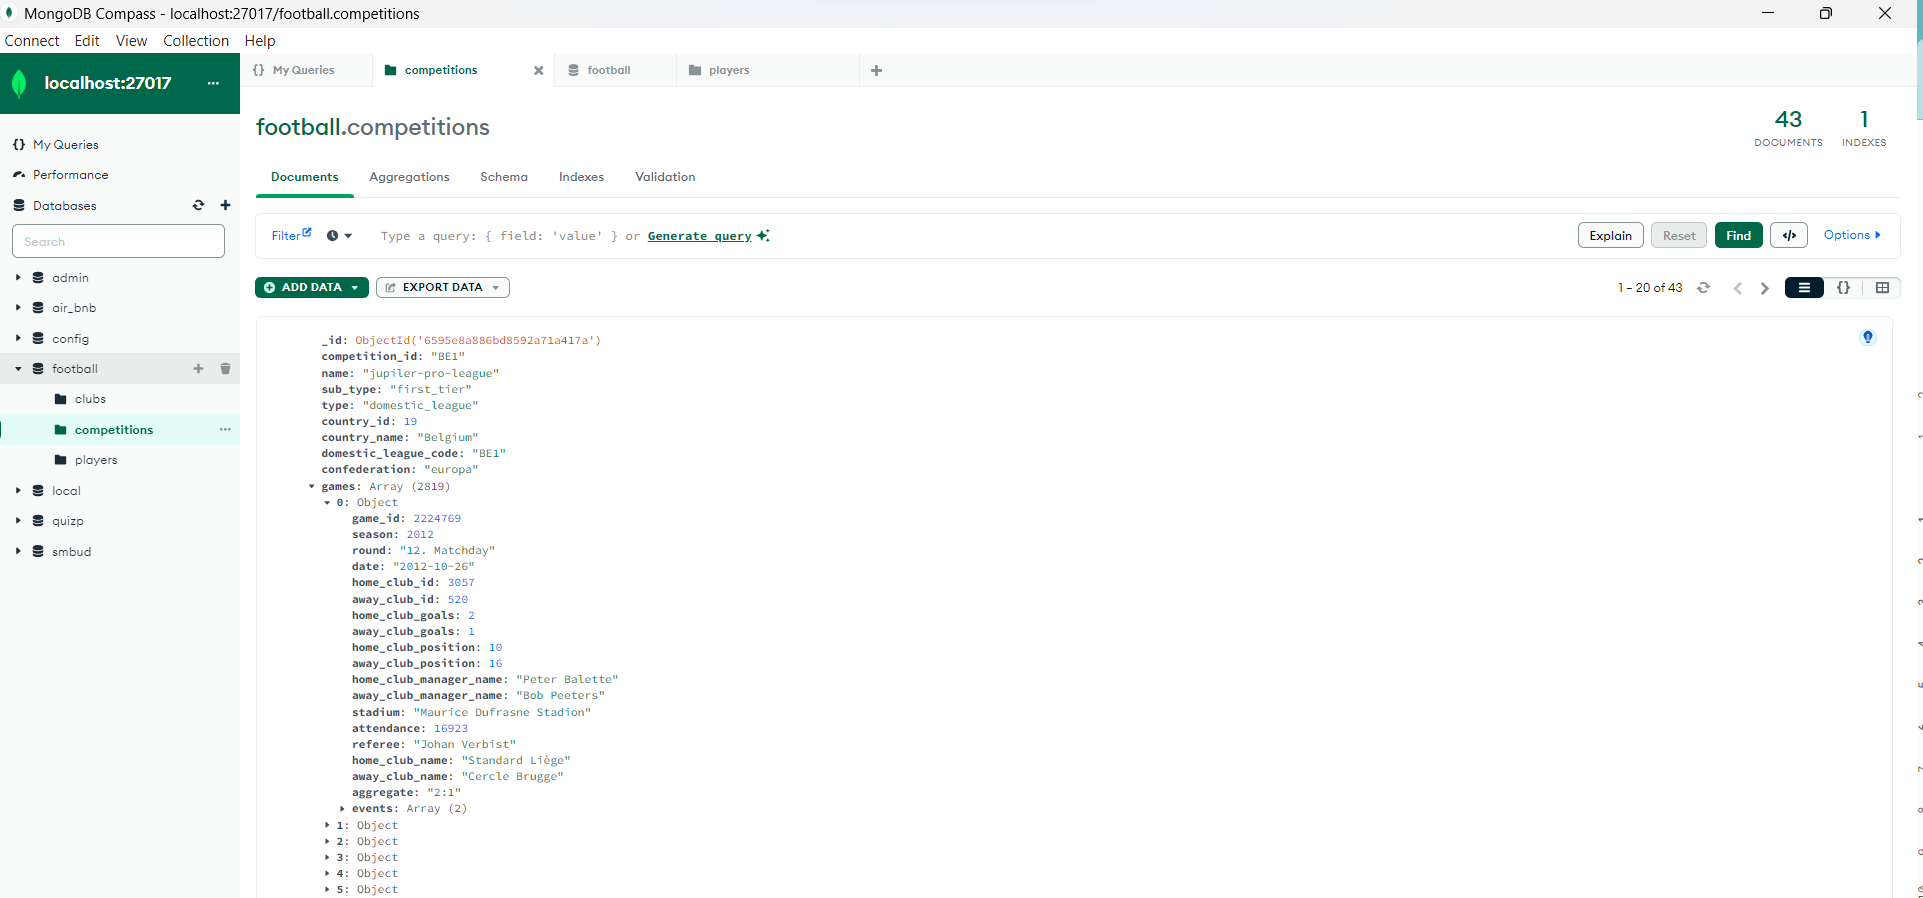
\includegraphics[scale=0.45]{Images/Dataset/competitions.png}
    \caption{Competitions Collection}
\end{figure}
\begin{tabular}{|l|l|p{8cm}|}
    \hline
    \textbf{Attribute}            & \textbf{Type}           & \textbf{Description} \\ \hline
    \_id                          & ObjectId                & A unique identifier for the document. \\ \hline
    competition\_id               & String                  & An identifier for the competition. \\ \hline
    name                          & String                  & The official name of the competition. \\ \hline
    sub\_type                     & String                  & A category within the competition, such as "first\_tier". \\ \hline
    type                          & String                  & The nature of the competition, for example, "domestic\_league". \\ \hline
    country\_id                   & Int32                   & A numeric identifier for the country associated with the competition. \\ \hline
    country\_name                 & String                  & The name of the country. \\ \hline
    domestic\_league\_cod         & String                  & A unique code representing the domestic league. \\ \hline
    confederation                 & String                  & The football confederation to which the competition belongs. \\ \hline
    games                         & Array                   & A collection of game records associated with the competition. \\ \hline
\end{tabular}
\subsubsection{Game Object inside Competition}
    \begin{tabular}{|l|l|p{8cm}|}
        \hline
        \textbf{Attribute}            & \textbf{Type}           & \textbf{Description} \\ \hline
    game\_id                      & Int32                   & The unique identifier for the game. \\ \hline
    season                        & Int32                   & The year of the football season. \\ \hline
    round                         & String                  & Distinct round: ['1. Matchday' '3. Matchday' '4. Matchday' '11. Matchday'  $\ldots$    \\ \hline
    date                          & String                  & When the game was played. \\ \hline
    home\_club\_id                & Int32                   & Identifier for the home club. \\ \hline
    away\_club\_id                & Int32                   & Identifier for the away club. \\ \hline
    home\_club\_goals             & Int32                   & Goals scored by the home club. \\ \hline
    away\_club\_goals             & Int32                   & Goals scored by the away club. \\ \hline
    home\_club\_position          & Int32                   & League position of the home club at game time. \\ \hline
    away\_club\_position          & Int32                   & League position of the away club at game time. \\ \hline
    home\_club\_manager\_name     & String                  & Name of the home club's manager. \\ \hline
    away\_club\_manager\_name     & String                  & Name of the away club's manager. \\ \hline
    stadium                       & String                  & Name of the stadium where the game was played. \\ \hline
    attendance                    & Int32                   & Number of people who attended the game. \\ \hline
    referee                       & String                  & Name of the referee of the game. \\ \hline
    home\_club\_name              & String                  & Name of the home club. \\ \hline
    away\_club\_name              & String                  & Name of the away club. \\ \hline
    aggregate                     & String                  & Overall score \\ \hline
    events                        & Array (of objects)      & An array detailing significant events during the game. \\ \hline
    \end{tabular}
\subsubsection{Events inside Games inside Competions}
\begin{tabular}{|l|l|p{8cm}|}
    \hline
    \textbf{Attribute}   & \textbf{Type}         & \textbf{Description} \\ \hline
    minute               & Int32                 & The match time in minutes when the event occurred. \\ \hline
    type                 & String                & The category of the event, e.g., "Substitutions” or “Goals” \\ \hline
    player\_id           & Int32                 & The unique identifier of the player involved in the event. \\ \hline
    description          & Null/String           & A detailed description of the event, if available. \\ \hline
    player\_in\_id       & Int32                 & The unique identifier of the player substituted into the game, relevant for substitution events. \\ \hline
    \end{tabular}





\subsection{Players}
\begin{figure}[htbp]
    \centering
    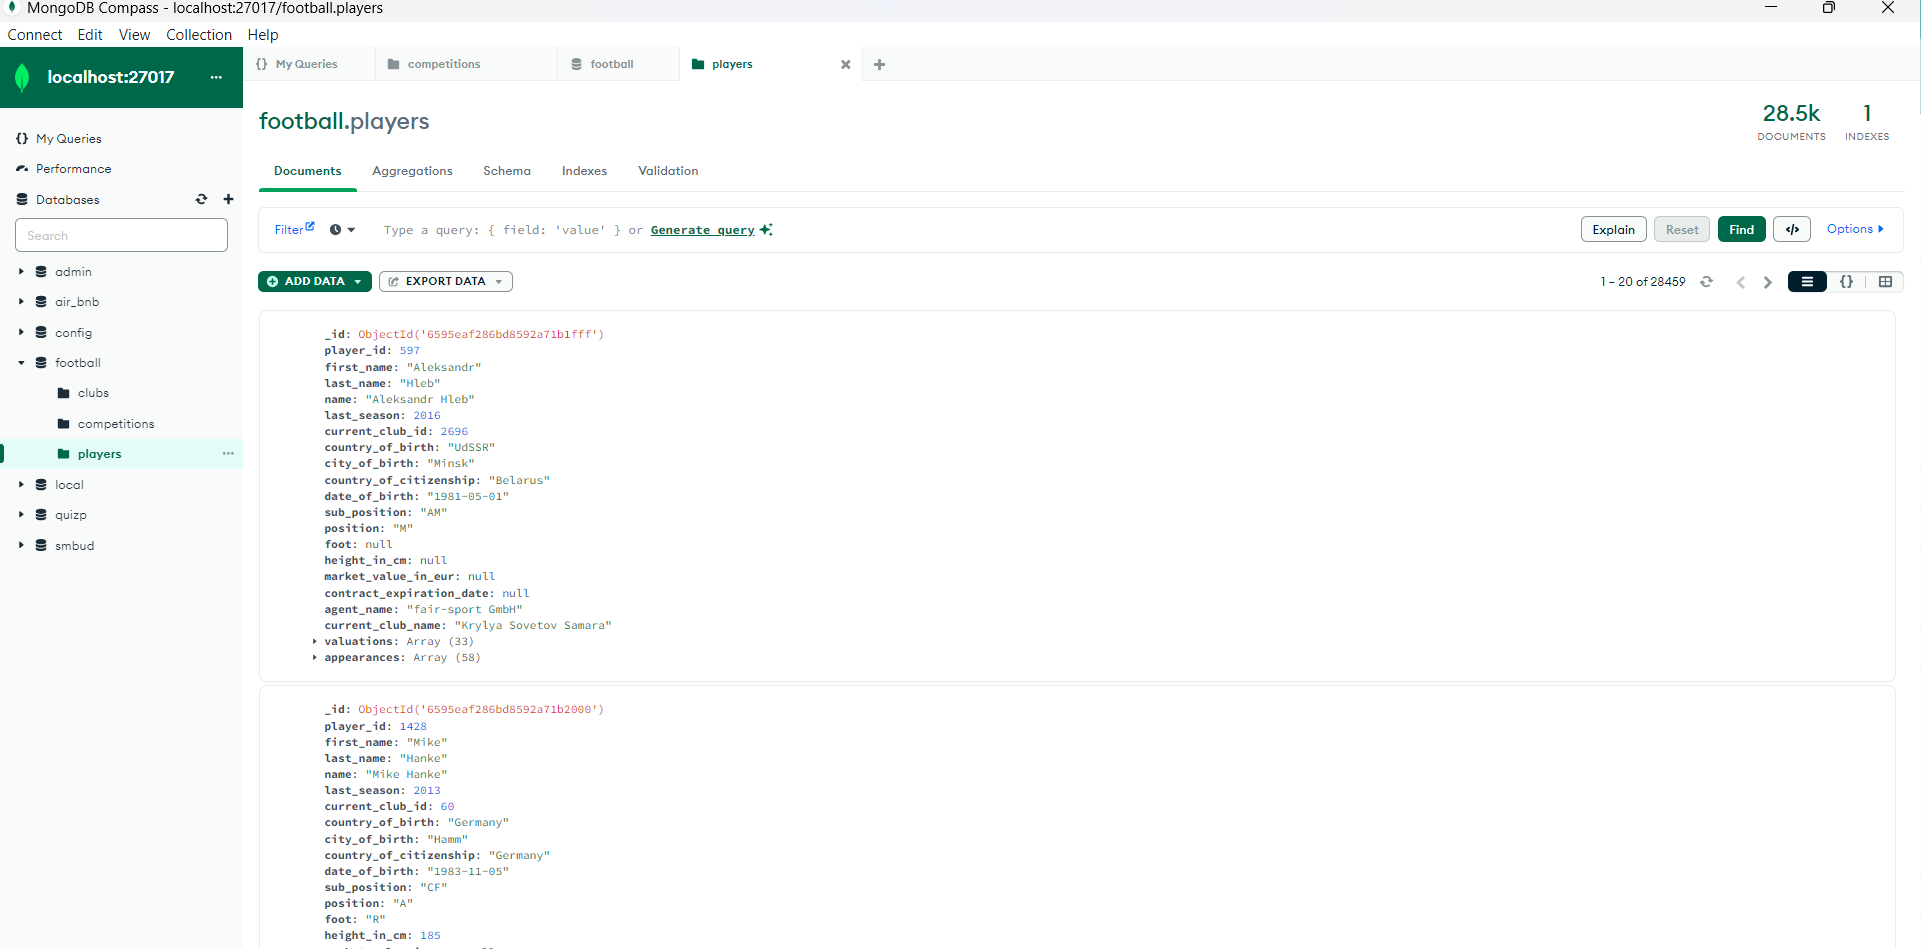
\includegraphics[scale=0.45]{Images/Dataset/players.png}
    \caption{Players Collection}
\end{figure}
\begin{tabular}{|l|l|p{8cm}|}
    \hline
    \textbf{Attribute}             & \textbf{Type}            & \textbf{Description} \\ \hline
    \_id                           & ObjectId                 & A unique identifier for the document. \\ \hline
    player\_id                     & Int32                    & A numeric identifier for the player. \\ \hline
    first\_name                    & String                   & The player's first name. \\ \hline
    last\_name                     & String                   & The player's surname. \\ \hline
    name                           & String                   & The full name of the player. \\ \hline
    last\_season                   & Int32                    & The last active season of the player. \\ \hline
    current\_club\_id              & Int32                    & Identifier for the player's current club. \\ \hline
    country\_of\_birth             & String                   & The country where the player was born. \\ \hline
    city\_of\_birth                & String                   & The city where the player was born. \\ \hline
    country\_of\_citizenship       & String                   & The country of the player's citizenship. \\ \hline
    date\_of\_birth                & String                   & The player's birthdate. \\ \hline
    sub\_position                  & String                   & The player's specific position on the field. \\ \hline
    position                       & String                   & The general position category the player occupies. \\ \hline
    foot                           & Null/String              & Preferred foot of the player. \\ \hline
    height\_in\_cm                 & Null/Int32               & The player's height in centimeters. \\ \hline
    market\_value\_in\_eur         & Null/Int32               & The player's market value in euros. \\ \hline
    contract\_expiration\_date     & String                   & When the player's contract is set to expire. \\ \hline
    agent\_name                    & String                   & The name of the player's agent. \\ \hline
    current\_club\_name            & String                   & The name of the player's current club. \\ \hline
    valuations                     & Array (of objects)       & A history of the player's market value evaluations. \\ \hline
    appearances                    & Array (of objects)       & A record of the player's appearances in games. \\ \hline
    \end{tabular}
\subsubsection{Player Valuations}
\begin{tabular}{|l|l|p{8cm}|}
    \hline
    \textbf{Attribute}             & \textbf{Type}           & \textbf{Description} \\ \hline
    last\_season                   & Int32                   & The season year of the valuation. \\ \hline
    market\_value\_in\_eur         & Int32                   & The player's market value in euros at that time. \\ \hline
    current\_club\_id              & Int32                   & The identifier for the club the player was with during that season. \\ \hline
    \end{tabular}
\subsubsection{Player Appearances}
\begin{tabular}{|l|l|p{8cm}|}
    \hline
    \textbf{Attribute}      & \textbf{Type}    & \textbf{Description} \\ \hline
    game\_id                & Int32            & The identifier for the game. \\ \hline
    date                    & String           & The date when the game was played. \\ \hline
    competition\_id         & String           & The identifier for the competition in which the game took place. \\ \hline
    yellow\_cards           & Int32            & The number of yellow cards received by the player in the game. \\ \hline
    red\_cards              & Int32            & The number of red cards received by the player in the game. \\ \hline
    goals                   & Int32            & The number of goals scored by the player in the game. \\ \hline
    assists                 & Int32            & The number of assists made by the player in the game. \\ \hline
    minutes\_played         & Int32            & The number of minutes the player played in the game. \\ \hline
    \end{tabular}

\chapter{Queries}
\section{Leagues analysed}
The competitions analyzed will include the Champions League and the major national leagues of Europe: Ligue 1 (France), LaLiga (Spain), Premier League (England), Serie A (Italy), and Bundesliga (Germany). The Champions League is Europe's most prestigious international competition, featuring Europe's best teams. The other national leagues are among the most important in Europe, characterized by top players, significant economic power of the clubs, and a high degree of competitiveness and visibility at the international level.

\begin{tabular}{|p{3cm}|p{2cm}|p{2cm}|p{2cm}|p{7cm}|}
    \hline
    \textbf{LEAGUE TYPE}          & \textbf{LEAGUE COUNTRY} & \textbf{LEAGUE CODE} & \textbf{LEAGUE NAME} & \\ \hline
    International (European) League &                        & CL                   & Champions League  & \\
    & & & &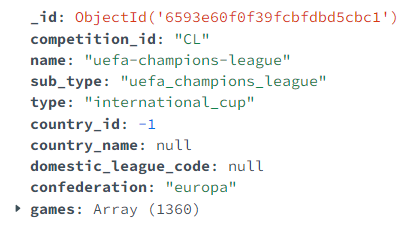
\includegraphics[scale=0.85]{Images/Leagues analysed/CL.png}   \\ \hline
    Domestic League                & FRANCE                 & FR1                  & Ligue1             & \\
    & & & &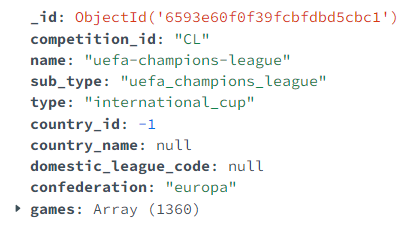
\includegraphics[scale=0.85]{Images/Leagues analysed/CL.png}  \\ \hline
    Domestic League                & SPAIN                  & ES1                  & LaLiga              & \\
    & & & &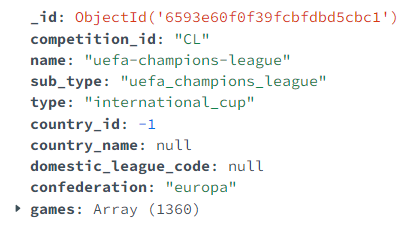
\includegraphics[scale=0.85]{Images/Leagues analysed/CL.png} \\ \hline
    \end{tabular}

    \begin{tabular}{|p{3cm}|p{2cm}|p{2cm}|p{2cm}|p{6cm}|}
        \hline
        \textbf{LEAGUE TYPE}          & \textbf{LEAGUE COUNTRY} & \textbf{LEAGUE CODE} & \textbf{LEAGUE NAME} & \\ \hline
    Domestic League                & ENGLAND                & GB1                  & Premier League     & \\
    & & & &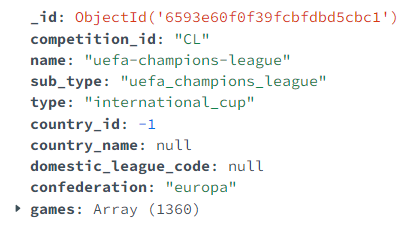
\includegraphics[scale=0.7]{Images/Leagues analysed/CL.png}  \\ \hline
    Domestic League                & GERMANY                & L1                   & Bundesliga         & \\
    & & & &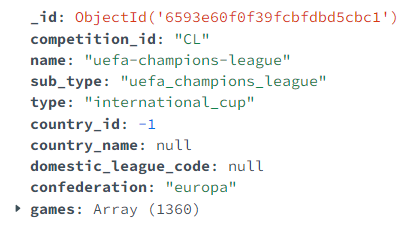
\includegraphics[scale=0.7]{Images/Leagues analysed/CL.png}  \\ \hline
    Domestic League                & ITALY                  & IT1                  & Serie A            & \\
    & & & &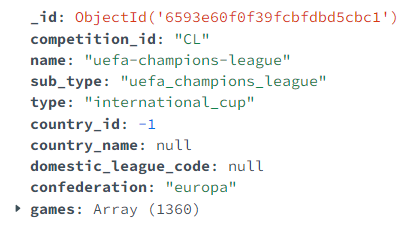
\includegraphics[scale=0.7]{Images/Leagues analysed/CL.png}  \\ \hline
\end{tabular}

\section{Players Collection}
\subsection{Top Football Agents}
This query lists agents according to the number of players they represent in the database, ordered from highest to lowest, clearly showing the most influential agents, or companies, in the world of football. In recent years, the figure of the agent or company, which looks after the interests of players, especially in terms of contracts, has had an enormous increase in power. \\
The agents or the most important companies manipulate the market trying to profit for the player but also for them: every transfer or contract in fact provides compensation for the agents.\\
In recent years, many agents have played the big game, cornering many clubs and earning huge amounts of money.\\
Simply, the query’s behavior is to group by the attribute agent\_name and then to compute the total players for each agent\_name.
\begin{verbatim}
    db.players.aggregate([
        { $match: { "agent_name": { $ne: null } } },
        { $group: { _id: "$agent_name", numberOfPlayers: { $sum: 1 } } }, 
        { $sort: { numberOfPlayers: -1 } }
      ])      
    \end{verbatim}
\begin{figure}[htbp]
    \centering
    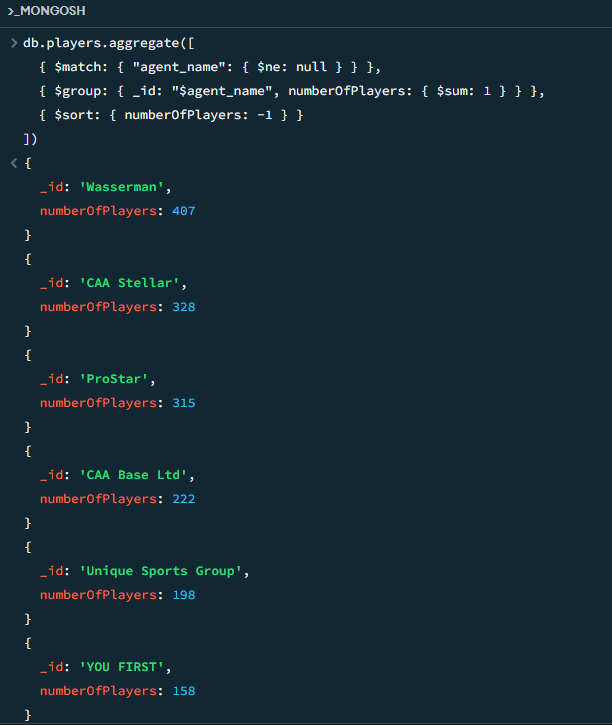
\includegraphics[scale=0.8]{Images/Queries/Top_Footbal_Agents/agents.png}
    \caption{Top Football Agents Result}
\end{figure}
\subsection{Competitions statistics}
Knowing the statistics of players in competitions is certainly important to identify those talents to be acquired during the football market phase. There are many characteristics that can be evaluated for a player: for example, his goals, assists, cards taken or minutes played in a specific competition.
There are many competitions around the world, but only the most important ones will be listed: the five top European leagues (England, Spain, France, Italy, Germany) and the Champions League.
\subsubsection{Top GoalScorers}
The most coveted record or award is surely to become the top scorer in a competition. This query shows the best champions, usually strikers, to have scored the most goals.
The query starts with \$unwind to break down the appearances array of each player document, then filters the appearances for a given competition\_id. Next, \$group aggregates the data by player, adding up the goals scored and capturing the player's name. Finally, \$sort and \$limit sort the players from highest to lowest number of goals and limit the output to the top 10. 
\begin{verbatim}
    db.players.aggregate([
  { $unwind: "$appearances" },
  { $match: { "appearances.competition_id": "<competition_id>" } },
  {
    $group: {
      _id: "$_id",
      totalGoals: { $sum: "$appearances.goals" },
      playerName: { $first: "$name" } // Assumi che 'name' sia il campo che contiene il nome del giocatore
      }
      },
      { $sort: { totalGoals: -1 } },
      { $limit: 10 }
    ])
    
\end{verbatim}
\begin{itemize}
    \item CL\\
        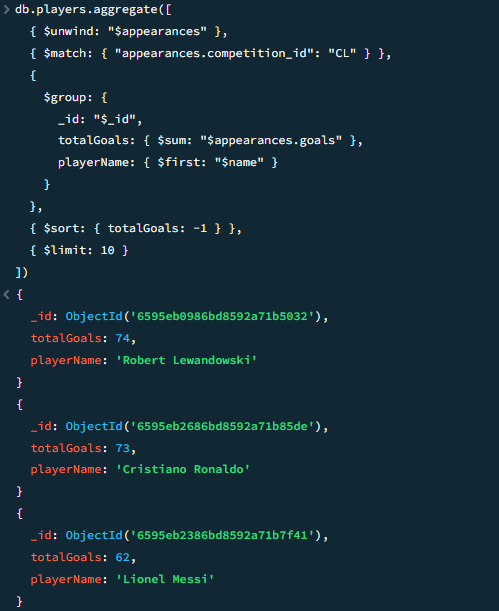
\includegraphics[scale=0.8]{Images/Queries/Competitions_statistics/top_goalscorers/CL.png}
    \item IT1\\
    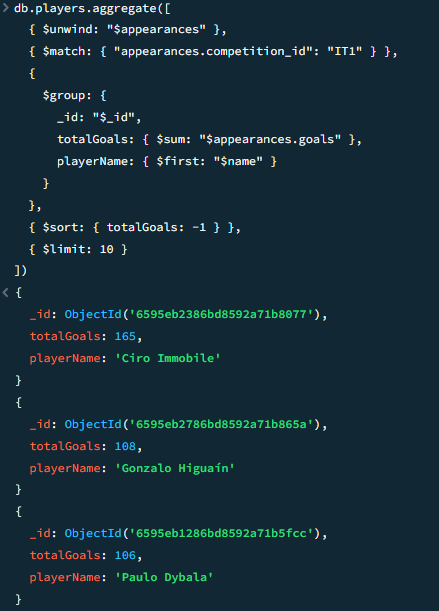
\includegraphics[scale=0.8]{Images/Queries/Competitions_statistics/top_goalscorers/IT1.png}
    \item ES1\\
    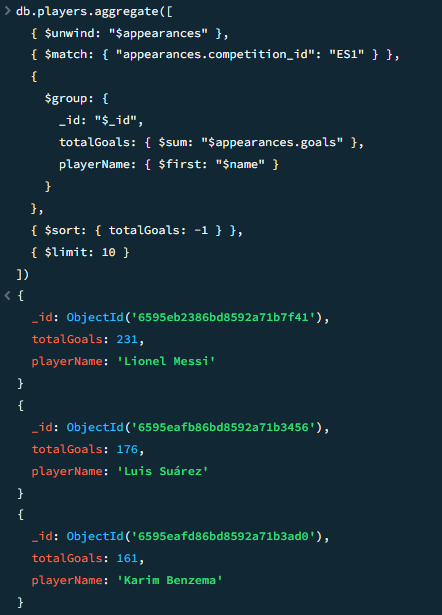
\includegraphics[scale=0.8]{Images/Queries/Competitions_statistics/top_goalscorers/ES1.png}
    \item FR1\\
    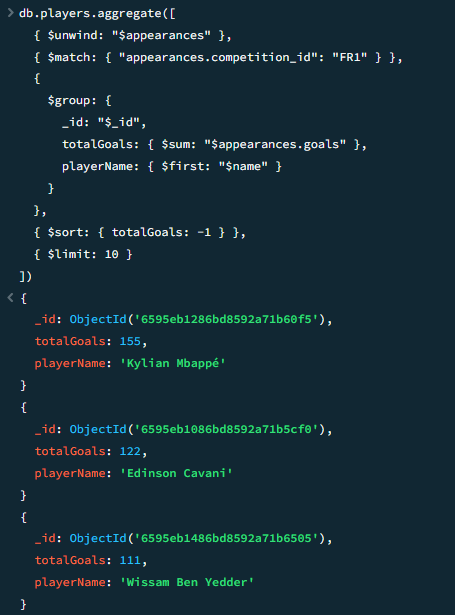
\includegraphics[scale=0.8]{Images/Queries/Competitions_statistics/top_goalscorers/FR1.png}
    \item GB1\\
    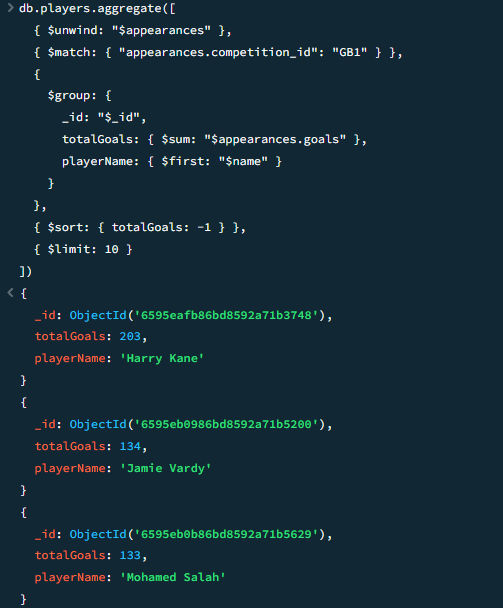
\includegraphics[scale=0.8]{Images/Queries/Competitions_statistics/top_goalscorers/GB1.png}
    \item L1\\
    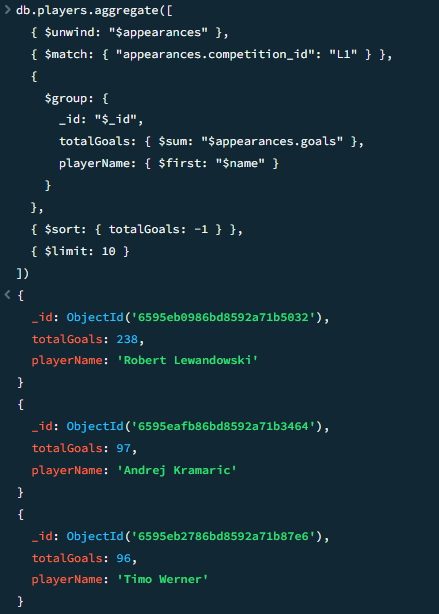
\includegraphics[scale=0.8]{Images/Queries/Competitions_statistics/top_goalscorers/L1.png}
\end{itemize}

\subsection{Best Assist-men}
Making an assist means putting a teammate in a position to put the ball in the net. This is also a very important statistic, often peculiar to side or full-back defenders, midfielders or wingers. The query starts with $unwind to break down the appearances array of each player document, then filters the appearances for a given competition_id. Next, $group aggregates the data by player, adding up the assists and capturing the player's name. Finally, there is a descending sort and a limit for the best 10 assist-men.

\begin{verbatim}
    db.players.aggregate([
  { $unwind: "$appearances" },
  { $match: { "appearances.competition_id": "<competition_id>" } },
  { 
    $group: {
      _id: "$_id",
      totalAssists: { $sum: "$appearances.assists" },
      playerName: { $first: "$name" } // Aggiunge il nome del giocatore
    }
  },
  { $sort: { totalAssists: -1 } },
  { $limit: 10 }
])

\end{verbatim}
\begin{figure}[htbp]
    \centering
    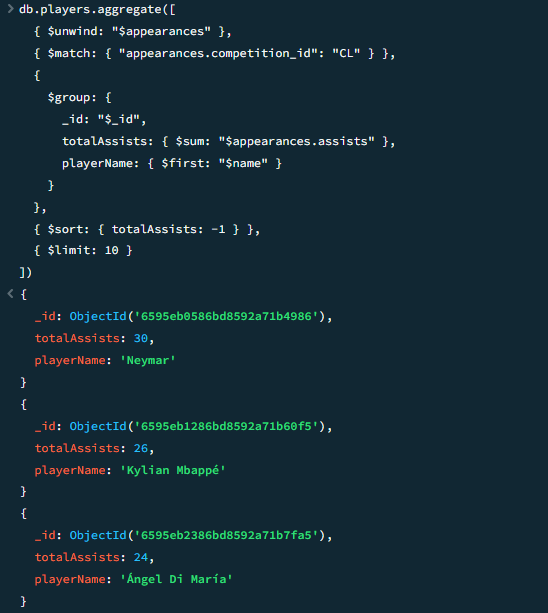
\includegraphics[scale=0.6]{Images/Queries/Competitions_statistics/best-assistmen/CL.png}
    \caption{Best Assist-men Executed with CL competition}
\end{figure}
\newpage
\subsection{Players with multiple yellow cards}
There are also many players who make impetuousness and confrontation their strong point. The statistics on yellow cards say a lot about those players who exploit their physical strength, but because of this attitude are prone to committing fouls, punishable by yellow cards. The query starts with $unwind to break down the appearances array of each player document, then filters the appearances for a given competition_id. Next, $group aggregates the data by player, adding up the yellow cards taken and showing the player's name. 
\begin{verbatim}
    db.players.aggregate([
  { $unwind: "$appearances" },
  { $match: { "appearances.competition_id": "<competition_id>" } },
  { $group: { _id: "$_id", totalYellowCards: 
  +{ $sum: "$appearances.yellow_cards" },  playerName: { $first: "$name" }  } },
  { $sort: { totalYellowCards: -1 } },
  { $limit: 10 }
])

\end{verbatim}

\begin{figure}[htbp]
    \centering
    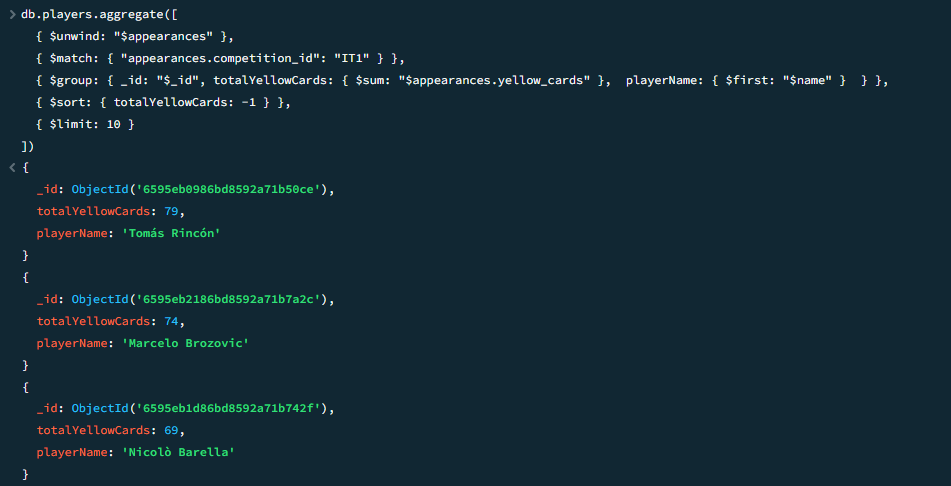
\includegraphics[scale=1]{Images/Queries/Competitions_statistics/yellow-cards/IT1.png}
    \caption{Players with multiple yellow cards Executed with IT1 competition}
\end{figure}
\newpage
\subsection{Players with multiple red cards}
In contrast to yellow cards, which can happen in the course of a match, getting a red card means, most of the time, having committed something serious, such as a bad foul, violent conduct or repeated protests to the referee. This statistic shows those players who struggle most to maintain control on the pitch and whose attitudes risk leaving the team one down. The query starts with $unwind to break down the appearances array of each player document, then filters the appearances for a given competition_id. Next, $group aggregates the data by player, adding up the red cards for each player. 
\begin{verbatim}
    db.players.aggregate([
  { $unwind: "$appearances" },
  { $match: { "appearances.competition_id": "<competition_id>" } },
  { $group: { _id: "$_id", totalRedCards: 
  { $sum: "$appearances.red_cards" }, playerName: { $first: "$name" } } },
  { $sort: { totalRedCards: -1 } },
  { $limit: 10 }
])
\end{verbatim}
\begin{figure}[htbp]
    \centering
    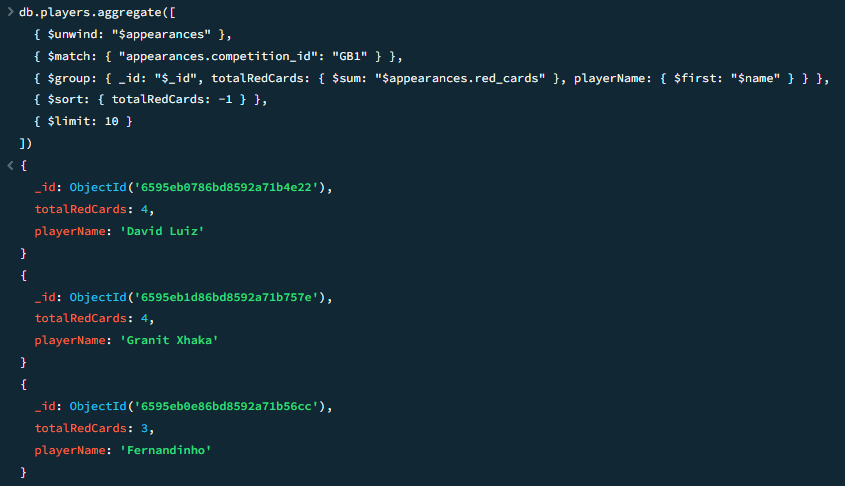
\includegraphics[scale=1]{Images/Queries/Competitions_statistics/red-cards/GB1.png}
    \caption{Players with multiple red cards Executed with IT1 competition}
\end{figure}

\subsection{Players with the most minutes played}
This analysis shows those players who are certainties for their clubs: the so-called immovable starters. These players, workaholics par excellence, are usually the players who are almost always at the top, avoiding injuries. The query breaks down appearances, then it filters the appearances in a certain league, and then sums up the minutes played by each player, showing also the name of him.
\begin{verbatim}
    db.players.aggregate([
        { $unwind: "$appearances" },
        { $match: { "appearances.competition_id": "<competition_id>" } },
        { $group: { _id: "$_id", totalMinutesPlayed: 
        { $sum: "$appearances.minutes_played" }, playerName: { $first: "$name" } } },
        { $sort: { totalMinutesPlayed: -1 } },
        { $limit: 10 }
      ])      
\end{verbatim}
\begin{figure}[htbp]
    \centering
    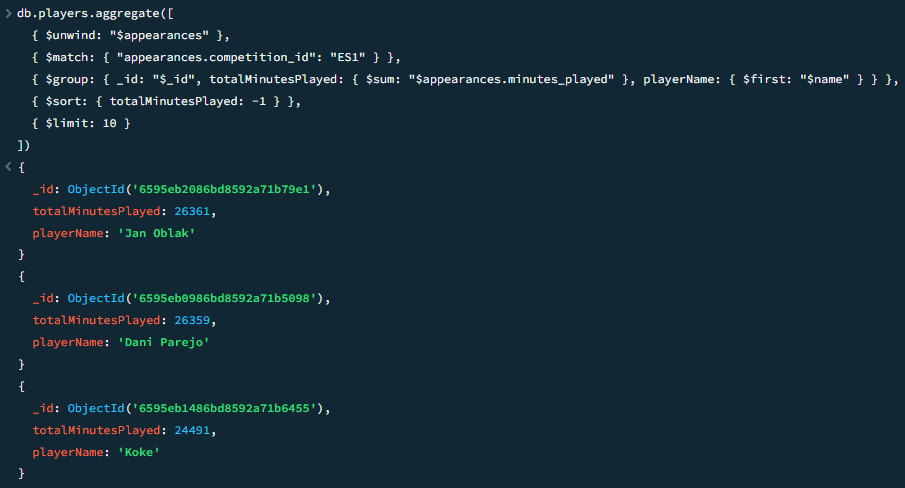
\includegraphics[scale=1]{Images/Queries/Competitions_statistics/minutes-played/ES1.png}
    \caption{Players with the most minutes played Executed with IT1 competition}
\end{figure}

\subsection{The players with the highest market value}
This query is designed to identify the top soccer players in the database, highlighting those with the highest market value. It provides an overview of the most valuable talents in the world of soccer, revealing the names of players who have not only demonstrated excellent performances on the field, but are also considered valuable investments in the soccer landscape. Players can sometimes be overestimated or underestimated. This data is important because it takes into account not only performance but also a player's age. Younger players with important statistics will command high market prices.
\\The first proposed query shows the current situation of market values for the players in the dataset ordered by their value in a descendent way.
\begin{verbatim}
db.players.find({},{ name: 1, market_value_in_eur: 1 }).sort(
    { market_value_in_eur: -1 }).limit(10)
\end{verbatim}
\begin{figure}[htbp]
    \centering
    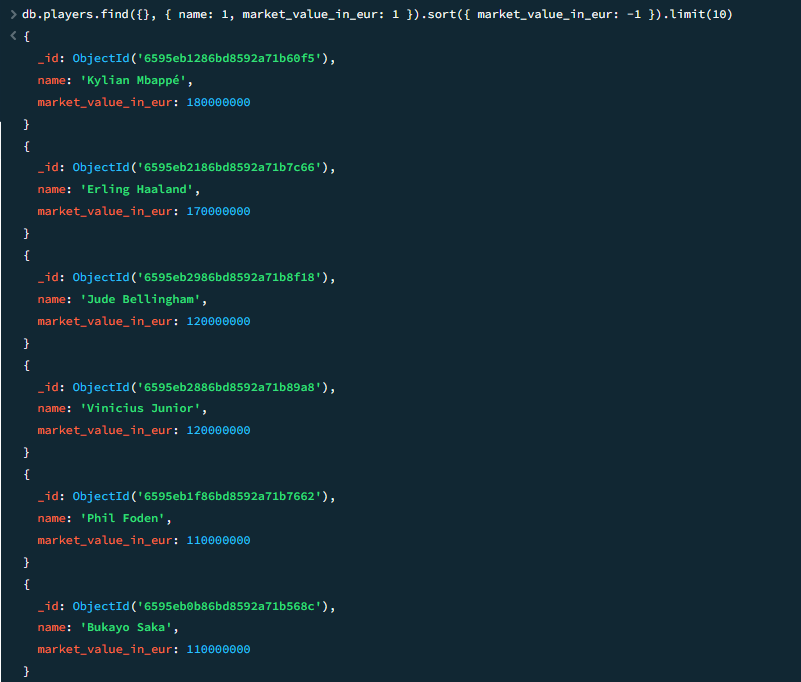
\includegraphics[scale=0.8]{Images/Queries/Highest_value_players/1.png}
    \caption{The players with the highest market value First Query Execution}
\end{figure}
The second query shows the best valuation for each player during its career and then orders these values in a descendent way.
\begin{verbatim}
    db.players.aggregate([
  { $unwind: "$valuations" },
  { $group: { _id: "$_id", name: { $first: "$name" }, maxMarketValue: 
    { $max: "$valuations.market_value_in_eur" }, season: 
        { $first: "$valuations.last_season" } } },
  { $sort: { maxMarketValue: -1 } }
])
\end{verbatim}
\begin{figure}[htbp]
    \centering
    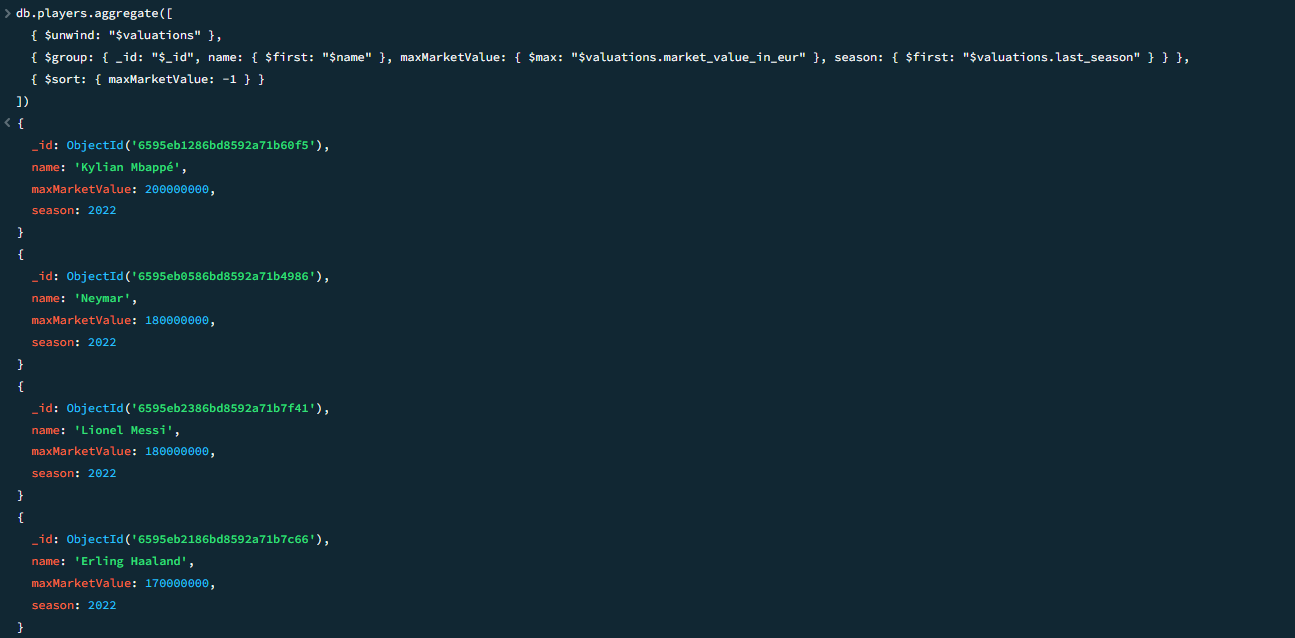
\includegraphics[scale=0.8]{Images/Queries/Highest_value_players/2.png}
    \caption{The players with the highest market value Second Query Execution}
\end{figure}

\subsection{The cities where the most players were born}
This query lists the cities that produced the most players. It uses the \$group operation to group players by their city of birth, counts the number of players for each city with \$sum, and then sorts the results descendingly to show which cities generated the most football talents.
\begin{verbatim}
db.players.aggregate([
  { $group: { _id: "$city_of_birth", numberOfPlayers: { $sum: 1 } } },
  { $sort: { numberOfPlayers: -1 } }
])
\end{verbatim}
Not all the players in the database have a city of birth, so there are a count also of the players with this attribute null.
\begin{figure}[htbp]
    \centering
    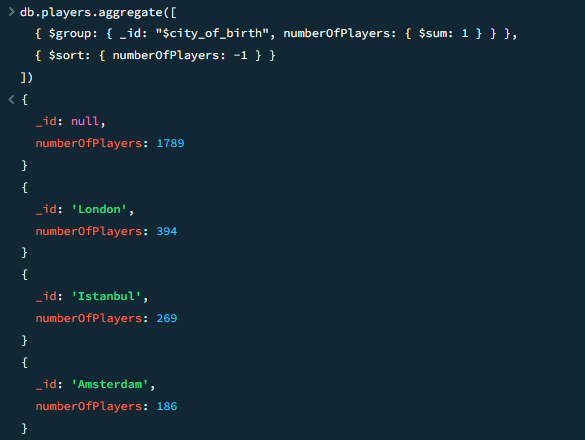
\includegraphics[scale=1]{Images/Queries/Cities/cities.png}
    \caption{The cities where the most players were born Query Execution}
\end{figure}
\subsection{The most prolific and expensive strikers}
This query aims to identify the center forwards (position "A") with the highest market value and the most goals scored. We start by filtering the players by their position, then use the \$unwind operator to decompose the array of appearances. Next, you aggregate the data to calculate the total number of goals and sort the results by market value and goals in a descending fashion. The first returned players are likely to be stars of the football. 
\begin{verbatim}
    db.players.aggregate([
        { $match: { position: "A" } },
        { $unwind: "$appearances" },
        { $group: { _id: "$_id", name: { $first: "$name" }, totalGoals: 
            { $sum: "$appearances.goals" }, marketValue: 
                { $first: "$market_value_in_eur" } } },
        { $sort: { marketValue: -1, totalGoals: -1 } }
      ])      
\end{verbatim}
\begin{figure}[htbp]
    \centering
    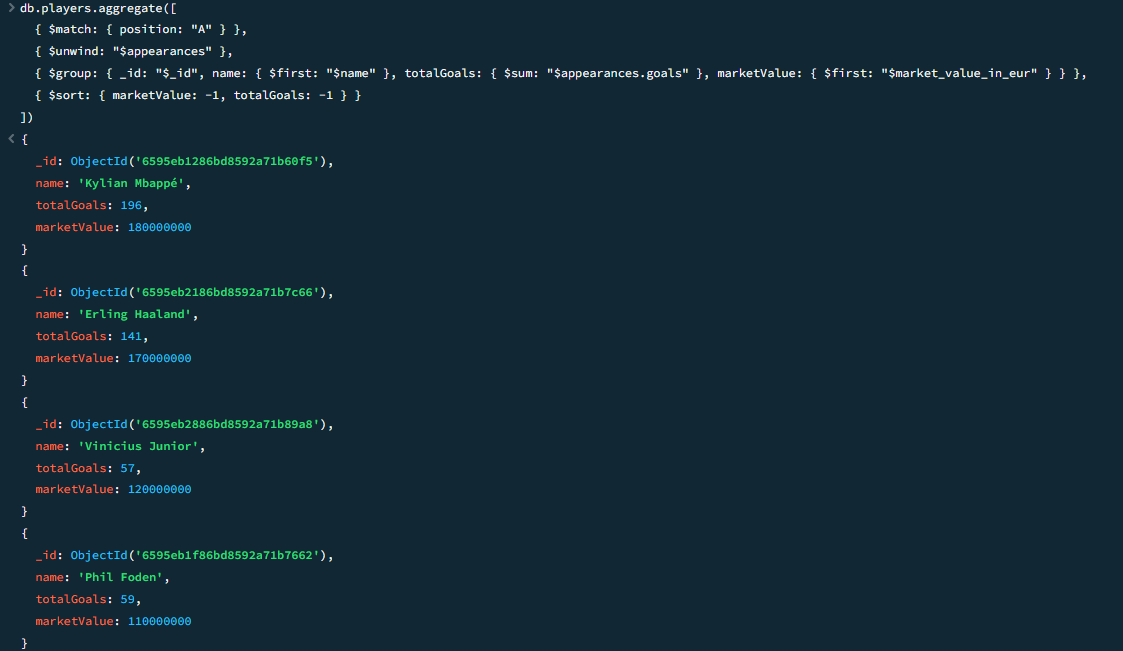
\includegraphics[scale=0.8]{Images/Queries/Prolific_expensive_strikers/pes.png}
    \caption{The most prolific and expensive strikers Query Execution}
\end{figure}
\subsection{Midfielders with the most goals and assists and a bounded valuation}
The query focuses on midfielders (position "M") with a market value lower and upper bound, but with a high number of goals and assists. After filtering by position, it uses \$unwind to decompose the array of appearances. It then aggregates the data to calculate the total goals and assists for each player, and finally sorts the results by goals and assists in descending order, taking into account only those players whose market value falls within a predefined average range. As can be understood, if a club has a certain budget available and wants to look for the best ones to fill a role, this query will be very useful.
\begin{verbatim}
    db.players.aggregate([
        { $match: { position: "M", market_value_in_eur:
         { $gte: 10000000, $lte: 20000000 } } },
        { $unwind: "$appearances" },
        { $group: { _id: "$_id", name: { $first: "$name" }, totalGoals: 
            { $sum: "$appearances.goals" }, totalAssists: 
                { $sum: "$appearances.assists" } } },
        { $sort: { totalGoals: -1, totalAssists: -1 } }
      ])    
      
    min=10000000
    max=20000000  
\end{verbatim}

\begin{figure}[htbp]
    \centering
    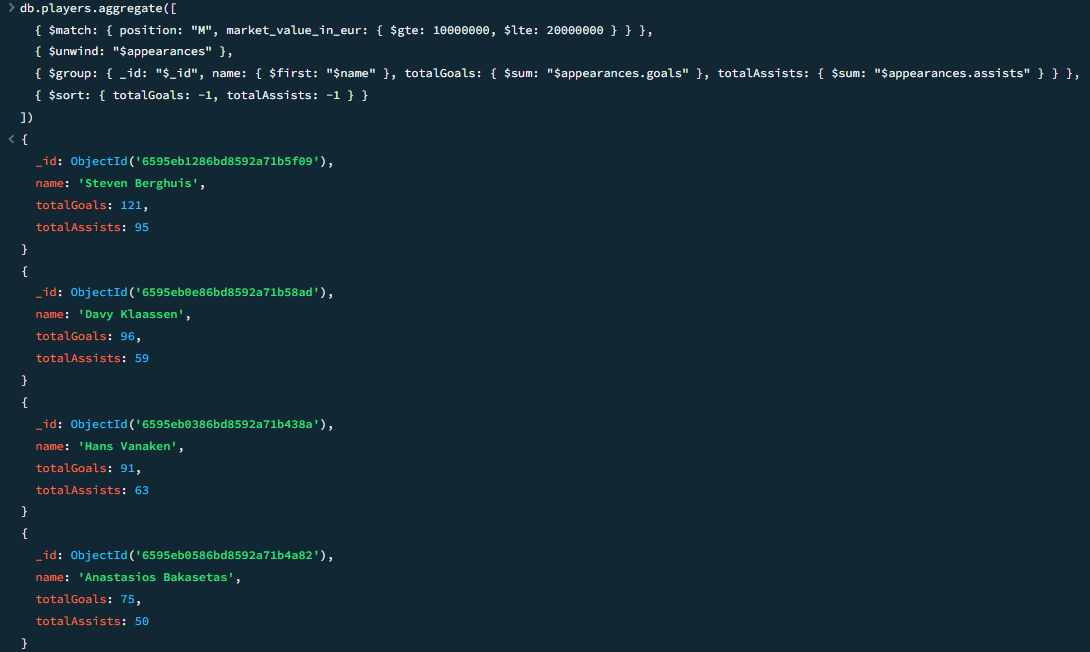
\includegraphics[scale=0.6]{Images/Queries/Midfielders_goal_assit_bounded_value/mgabv.png}
    \caption{Midfielders with the most goals and assists and a bounded valuation Query Execution}
\end{figure}

\subsection{The cheapest but most prolific full-back defenders}
This query aims to identify right-backs (RB) and left-backs (LB) with the lowest market value but high assists and goals. It filters players by RB and LB sub-positions, calculates the total assists and goals, and sorts first by ascending market value and then by descending assists and goals. The query highlights those full-backs who, while not having a high market value, have a significant impact in terms of their contribution to the game. Despite being defenders, offensive-minded teams need these players to increase their number of goals.

\begin{verbatim}
    db.players.aggregate([
        { $match: { 
            sub_position: { $in: ["RB", "LB"] },
            market_value_in_eur: { $ne: null }    }},
        { $unwind: "$appearances" },
        { $group: { 
            _id: "$_id", 
            name: { $first: "$name" },
            marketValue: { $first: "$market_value_in_eur" },
            totalAssists: { $sum: "$appearances.assists" },
            totalGoals: { $sum: "$appearances.goals" }
        }},
        { $sort: { marketValue: 1, totalAssists: -1, totalGoals: -1 } }
      ])
      
\end{verbatim}
\begin{figure}[htbp]
    \centering
    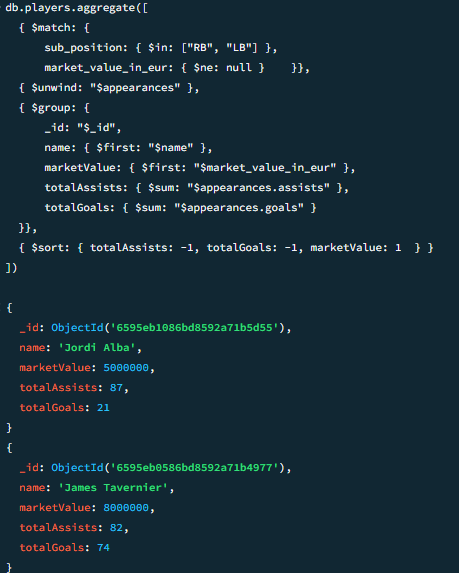
\includegraphics[scale=0.8]{Images/Queries/Cheapest_prolific_full_backs/cpfb.png}
    \caption{The cheapest but most prolific full-back defenders Query Execution}
\end{figure}

\subsection{Players in a Specific Match}
This aggregation query lists all players who appeared in a specific match, identified by the game\_ID. It begins by deconstructing the appearances array with \$unwind. Then, it filters the documents with \$match to only those where the game\_id within appearances matches the given ID. Finally, \$project is used to exclude the valuations field from the output, returning all other player details. This query is helpful for analyzing participation in particular games. In the case of this query the game:id chosen was 2469936 (of course it could be changed).

\begin{verbatim}
    db.players.aggregate([
  { $unwind: "$appearances" },
  { $match: { "appearances.game_id": 2469936 } },
  { $project:  { valuations: 0 } }
])
\end{verbatim}
\begin{figure}[htbp]
    \centering
    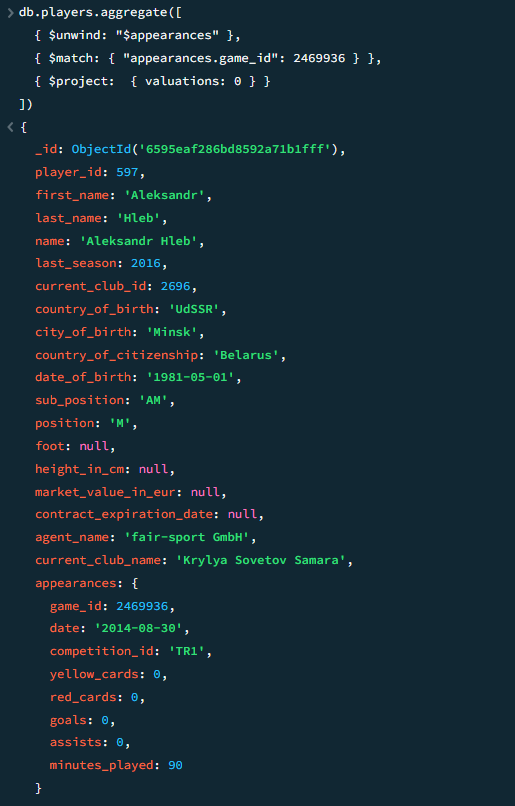
\includegraphics[scale=0.8]{Images/Queries/Players_in_game/pg.png}
    \caption{Players in a Specific Match Query Execution}
\end{figure}

\subsection{Defender with most cards (Yellow and Red cards summed up)}
This query identifies the defenders who received the highest total number of cards, summing yellow and red cards. After filtering players by defensive position, the query breaks down the array of appearances, aggregates the total number of red and yellow cards per player, and finally sorts the results in descending order to display the most "undisciplined" defenders.
\begin{verbatim}
    db.players.aggregate([
  { $match: { position: "D" } },
  { $unwind: "$appearances" },
  { $group: { _id: "$_id", name: { $first: "$name" }, totalCards: 
  { $sum: { $add: 
    ["$appearances.yellow_cards", "$appearances.red_cards"] } } } },
  { $sort: { totalCards: -1 } }
])
\end{verbatim}

\begin{figure}[htbp]
    \centering
    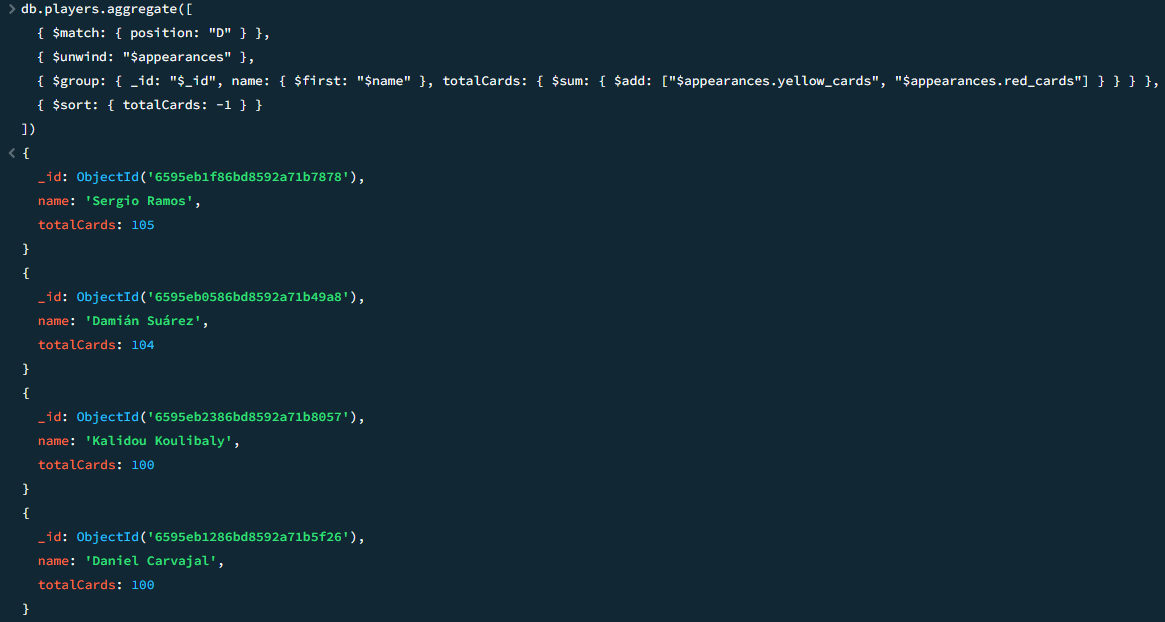
\includegraphics[scale=0.8]{Images/Queries/Defenders_most_cards/dmc.png}
    \caption{Defender with most cards  Query Execution}
\end{figure}

\subsection{The nations with the best talents in terms of market value during the years}
This query identifies the nations that produce the players with the highest market values by analyzing the maximum market value achieved by each player. After decomposing the valuations array, it aggregates the maximum market value for each player and then averages these maximum values by nation, sorting the nations by this average.
\begin{verbatim}
    db.players.aggregate([
  { $unwind: "$valuations" },
  { $group: { _id: "$_id", country: 
    { $first: "$country_of_citizenship" }, maxMarketValue:
     { $max: "$valuations.market_value_in_eur" } } },
  { $group: { _id: "$country", averageMaxMarketValue: 
    { $avg: "$maxMarketValue" } } },
  { $sort: { averageMaxMarketValue: -1 } }
])
\end{verbatim}
\begin{figure}[htbp]
    \centering
    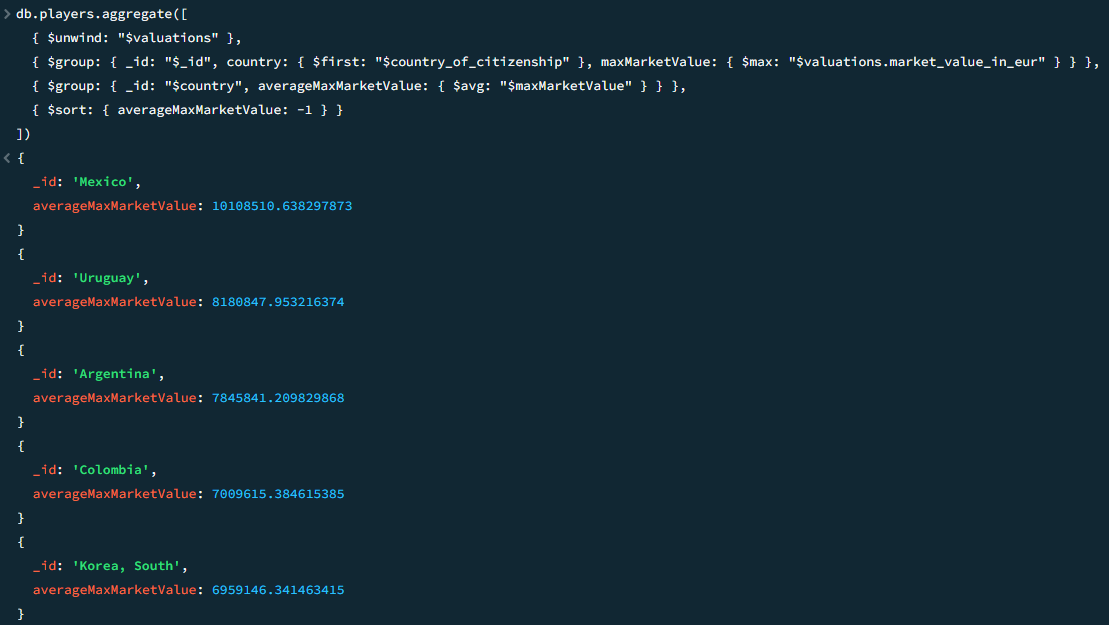
\includegraphics[scale=0.8]{Images/Queries/Nation_talents_market_value/ntmv.png}
    \caption{Nations with the best talents in terms of market value Query Execution}
\end{figure}

\subsection{The nations with most goals scored by their players}
This query identifies the nation that produces the players with the most goals. It first breaks down the array of each player's appearances, then groups the players by nation and adds up the goals scored. Finally, it sorts the nations by total number of goals to find out which nation produced the best scorers.
\begin{verbatim}
    db.players.aggregate([
  { $unwind: "$appearances" },
  { $group: { _id: "$country_of_citizenship", totalGoals: 
    { $sum: "$appearances.goals" } } },
  { $sort: { totalGoals: -1 } }
])
\end{verbatim}

\begin{figure}[htbp]
    \centering
    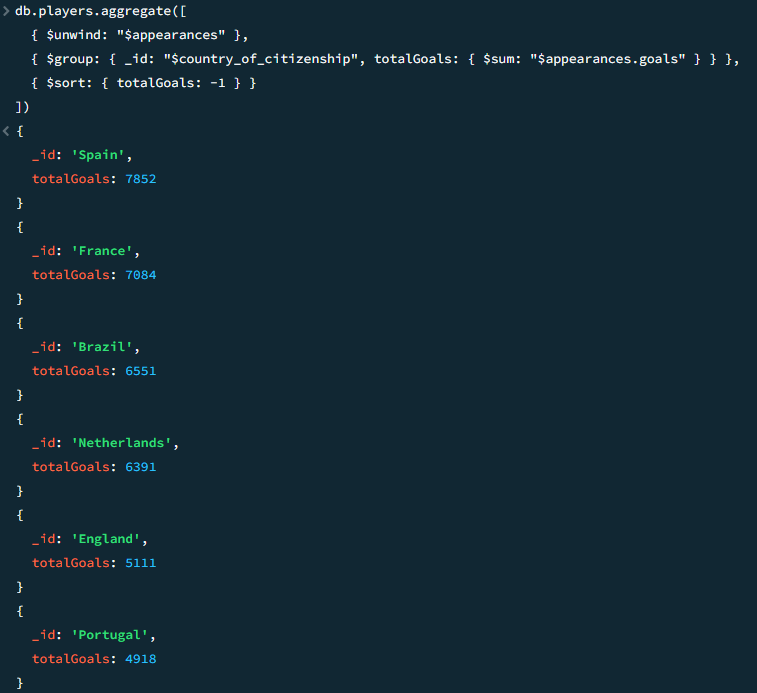
\includegraphics[scale=0.8]{Images/Queries/Nation_goals/ng.png}
    \caption{Nations with most goals scored by their players Query Execution}
\end{figure}

\subsection{Average Market Value for each club}

This query calculates the average market value of the players for each club. It uses the \$group operation to group players by their current club, then calculates the average market value (found in the valuations array) for each club. Finally, sort the results to show the clubs by the average market value of their players.

\begin{verbatim}
    db.players.aggregate([
  { $unwind: "$valuations" },
  { $group: { _id: "$current_club_name", averageMarketValue: 
    { $avg: "$valuations.market_value_in_eur" } } },
  { $sort: { averageMarketValue: -1 } }
])

\end{verbatim}

\begin{figure}[htbp]
    \centering
    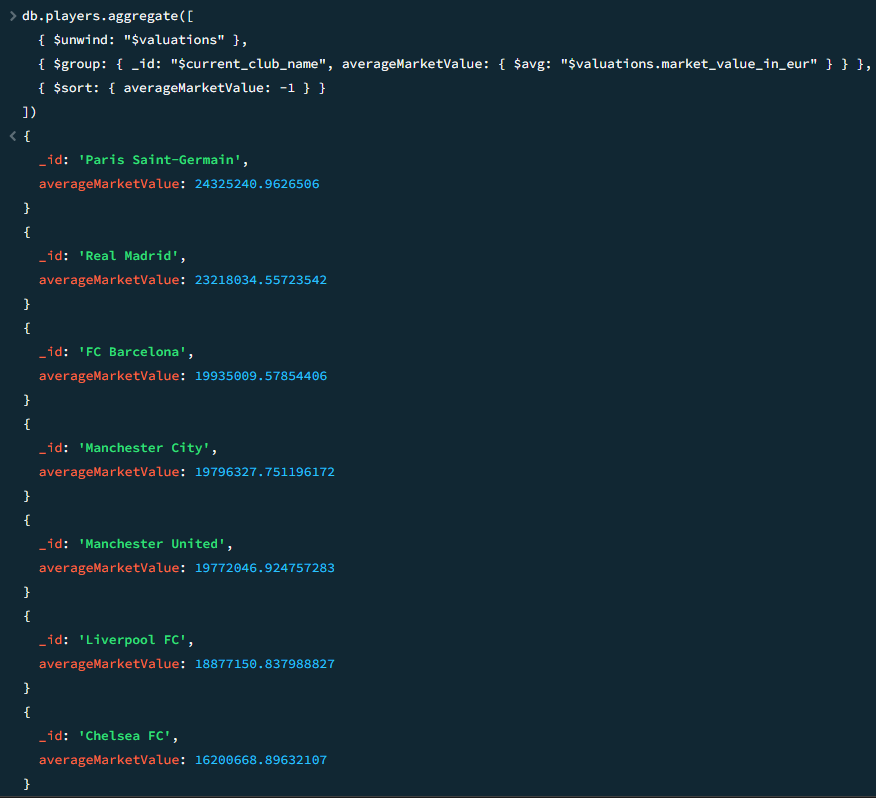
\includegraphics[scale=0.8]{Images/Queries/Average_market_value_club/amvc.png}
    \caption{Average Market Value for each club Query Execution}
\end{figure}

\subsection{Most Prolific free agents}

This query identifies free agent players with the best goal scoring statistics in the last season played. It starts by filtering players without a current club (free agent), then examines their performance in the last season, summing the total number of goals scored. Finally, it sorts the results to show the best scorers among free agents. Many teams resort to signing players without contracts to save on transfer costs, paying only contract fees and some fees to agents or at signing.

\begin{verbatim}
    db.players.aggregate([
  { $match: { current_club_name: null } },
  { $unwind: "$appearances" },
  { $group: { _id: "$_id", name: { $first: "$name" }, totalGoals: 
    { $sum: "$appearances.goals" }, lastSeason: 
        { $max: "$appearances.last_season" } } },
  { $sort: { totalGoals: -1 } }
])

\end{verbatim}

\begin{figure}[htbp]
    \centering
    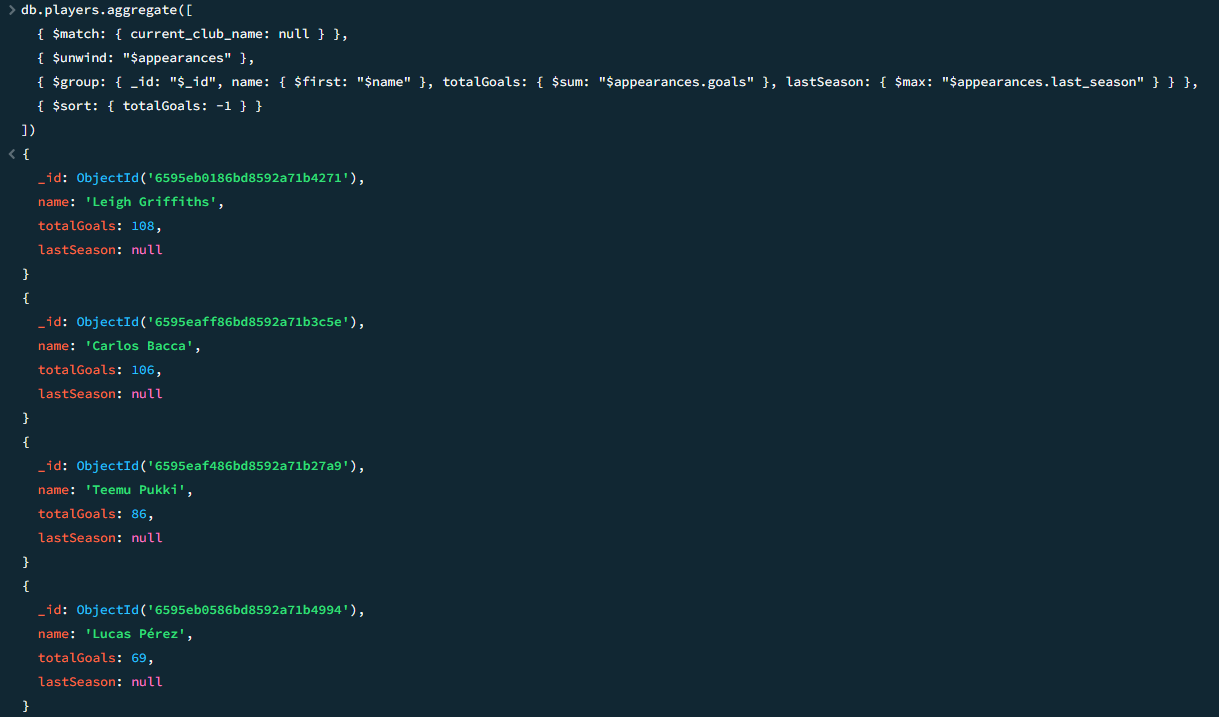
\includegraphics[scale=0.8]{Images/Queries/Most_prolific_free_agents/mpfa.png}
    \caption{Most Prolific free agents Query Execution}
\end{figure}


\subsection{Cristiano Ronaldo (specific player) goals }
To calculate the total number of goals scored by Cristiano Ronaldo, the query should first locate the specific player in the database (e.g., by name or unique ID). Next, it uses $unwind to decompose the array of appearances and $group to sum the goals scored. Finally, it presents the total goals.
Obviously, by changing names and searching for another player, one can see how many goals the requested player has scored.
\begin{verbatim}
    db.players.aggregate([
  { $match: { name: "Cristiano Ronaldo" } },
  { $unwind: "$appearances" },
  { $group: { _id: "$_id", totalGoals: { $sum: "$appearances.goals" } } }
])
\end{verbatim}
\begin{figure}[htbp]
    \centering
    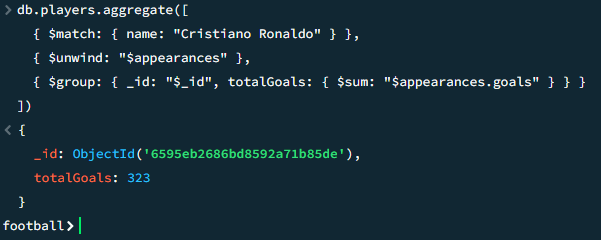
\includegraphics[scale=1]{Images/Queries/Cristiano_Ronaldo_goals/CRG.png}
    \caption{Cristiano Ronaldo Query Execution}
\end{figure}

\subsection{The youngest player}
To find the youngest player in the database, the query sorts all players by their date of birth, from newest to oldest. In this way, the first player in the resulting list will be the youngest. Of course, to find the oldest you need to change "-1" with "1".
\begin{verbatim}
    db.players.find().sort({ date_of_birth: -1 }).limit(1)
\end{verbatim}

\begin{figure}[htbp]
    \centering
    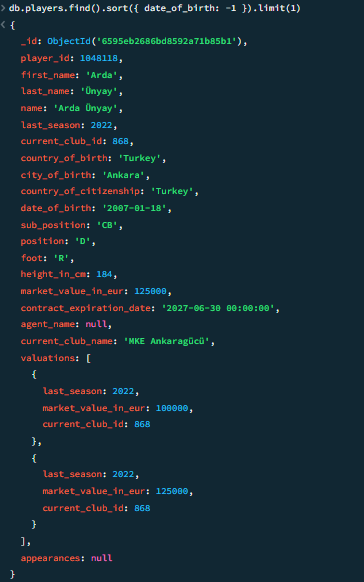
\includegraphics[scale=1]{Images/Queries/Youngest/y.png}
    \caption{The youngest player Query Execution}
\end{figure}

\subsection{Strikers with more matches without goals}
This query identifies the forwards who had the most appearances in games without scoring goals. It first filters by position, identifying forwards, then breaks down the array of appearances. With an aggregation, it counts the number of games in which the player did not score, and finally sorts the results to show who had the most appearances without scoring goals. 
\begin{verbatim}
    db.players.aggregate([
  { $match: { sub_position: "CF" } },
  { $unwind: "$appearances" },
  { $group: { _id: "$_id", name: { $first: "$name" },
    appearancesWithoutGoals: 
        { $sum: { $cond: [{ $eq: ["$appearances.goals", 0] }, 1, 0] } } } },
  { $sort: { appearancesWithoutGoals: -1 } }
])
\end{verbatim}

\begin{figure}[htbp]
    \centering
    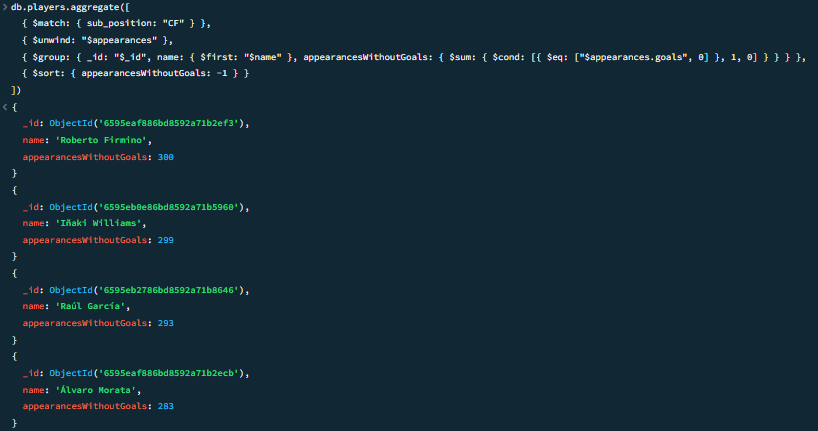
\includegraphics[scale=1]{Images/Queries/Strikers_without_goals/swg.png}
    \caption{Strikers with more matches without goals Query Execution}
\end{figure}

\subsection{Average height of goalkeepers}
Within the 'players' collection SI first filters by position, selecting only players classified as goalkeepers (e.g., position "G" for goalkeeper), then groups the data to calculate the average height.
\begin{verbatim}
    db.players.aggregate([
  { $match: { position: "G" } },  
  { $group: { _id: null, averageHeight: { $avg: "$height_in_cm" } } }
])
\end{verbatim}

\begin{figure}[htbp]
    \centering
    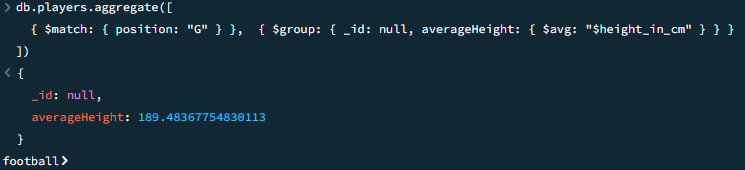
\includegraphics[scale=1]{Images/Queries/Avg_goalkeepers_height/agh.png}
    \caption{Average height of goalkeepers Query Execution}
\end{figure}

\subsection{Agent with the most valuable player}
This query identifies the agent of the player with the highest market value recorded directly in the player's document. Each player is assumed to have a market value defined in the market\_value\_in\_eur field. The query sorts all player documents by this value in a descending manner and selects the first document, which represents the player with the highest value, and then projects the name of the agent.

\begin{verbatim}
    db.players.find(
  { market_value_in_eur: { $exists: true, $ne: null } },
  { name: 1, agent_name: 1, market_value_in_eur: 1 }
).sort({ market_value_in_eur: -1 }).limit(1)
\end{verbatim}

\begin{figure}[htbp]
    \centering
    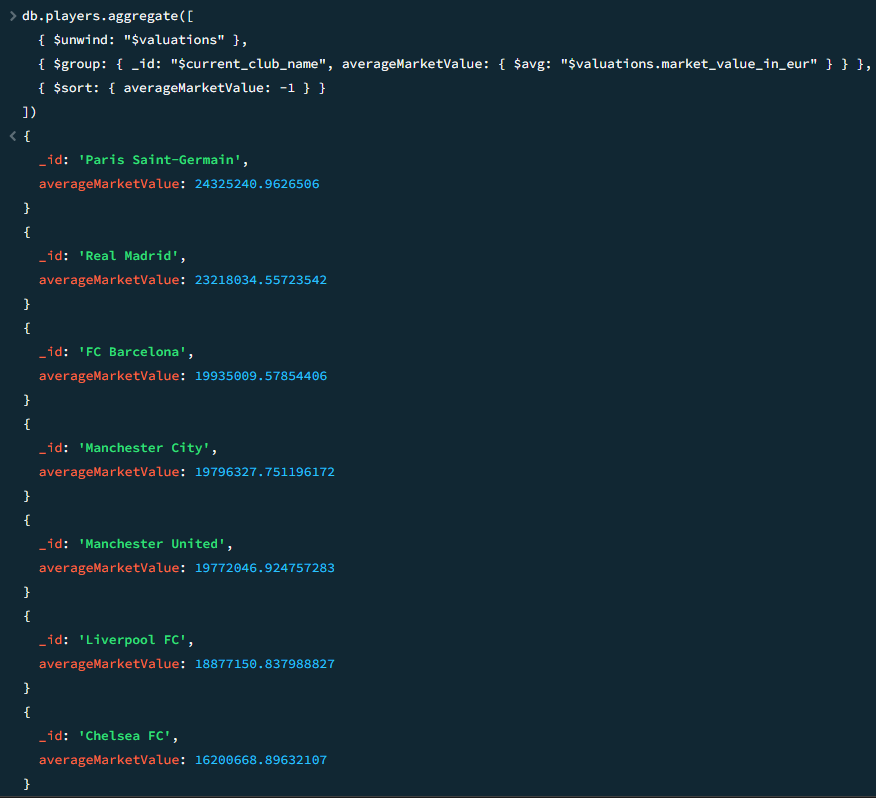
\includegraphics[scale=1]{Images/Queries/Average_market_value_club/amvc.png}
    \caption{Agent with the most valuable player Query Execution}
\end{figure}
However, in this specific case, the result will show "null" for the agent\_name field indicating that there is no registered agent, which may correspond to situations where a family member, such as the mother in Mbappé's case, assists the player in contractual matters.

\subsection{The italian players with the highest goal ratio}

This query shows the best italian players with the highest ratio between goal and appearances.
To get the Italian players with the highest goal-to-presence ratio, the query would first calculate the total goals and total appearances for each Italian player, then divide the total goals by the total number of appearances to get the ratio. Here is how it would be structured:

\begin{enumerate}
    \item Filter players by country\_of\_citizenship set to "Italy."
    \item Expand the appearances array.
    \item Group the results by player, adding up the goals scored and counting the appearances.
    \item Calculate the goals/appearances ratio for each player.
    \item Sort the results by goal/attendance ratio in a descending manner.
\end{enumerate}
The statistics are important only for players with more than 50 appearances.

\begin{verbatim}
    db.players.aggregate([
  { $match: { country_of_citizenship: "Italy" } },
  { $unwind: "$appearances" },
  { $group: { 
      _id: "$_id", 
      name: { $first: "$name" }, 
      totalGoals: { $sum: "$appearances.goals" }, 
      totalAppearances: { $sum: 1 }
    } 
  },
  { $match: { totalAppearances: { $gte: 50 } } },
  { $project: { 
      name: 1, 
      goalRatio: { $divide: [ "$totalGoals", "$totalAppearances" ] }
    } 
  },
  { $sort: { goalRatio: -1 } }
])
\end{verbatim}

\begin{figure}[htbp]
    \centering
    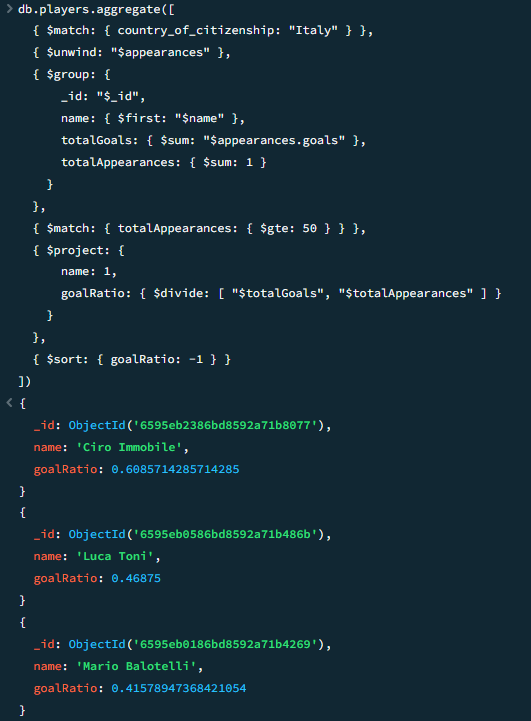
\includegraphics[scale=1]{Images/Queries/Italian_ratio_goals/irg.png}
    \caption{The italian players with the highest goal ratio Query Execution}
\end{figure}

\subsection{The French players with the highest minutes ratio}
This query shows the best italian players with the highest ratio between minutes and appearances.
To get the French players with the highest minutes-to-apperance ratio, the query would first calculate the total minutes and total appearances for each player, then divide the total minutes by the total number of appearances to get the ratio. Here is how it would be structured:
\begin{enumerate}
    \item Filter players by country\_of\_citizenship set to "France."
    \item Expand the appearances array.
    \item Group the results by player, adding up the minutes played and counting the appearances.
    \item Calculate the minutes/appearances ratio for each player.
    \item Sort the results by minutes/attendance ratio in a descending manner.
    \item The statistics are important only for players with more than 50 appearances.
\end{enumerate}
\begin{verbatim}
    db.players.aggregate([
  { $match: { country_of_citizenship: "France" } },
  { $unwind: "$appearances" },
  { $group: { 
      _id: "$_id", 
      name: { $first: "$name" }, 
      totaMinutes: { $sum: "$appearances.minutes_played" }, 
      totalAppearances: { $sum: 1 }
    } 
  },
  { $match: { totalAppearances: { $gte: 50 } } },
  { $project: { 
      name: 1, 
      minutesRatio: { $divide: [ "$totaMinutes", "$totalAppearances" ] }
    } 
  },
  { $sort: { minutesRatio: -1 } }
])
\end{verbatim}
\begin{figure}[htbp]
    \centering
    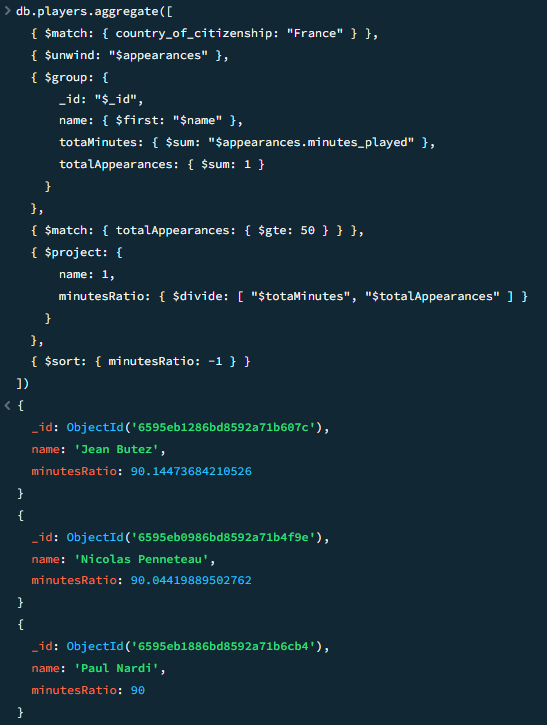
\includegraphics[scale=1]{Images/Queries/French_minutes_ratio/fmr.png}
    \caption{The French players with the highest minutes ratio Query Execution}
\end{figure}

\section{Competitions Collection }
\subsection{Most Followed Matches}
The query selects the games from the 'competitions' collection that had the most spectators. It uses the 'attendance' field within the array of 'games' for each competition. The goal is to identify those games that attracted the most significant audience attention, an indicator of the match's popularity or importance. 
The first query returns the most followed matches among all the competitions.
\begin{verbatim}
    db.competitions.aggregate([
  { $unwind: "$games" },
  { $project: 
    { "game_id": "$games.game_id", "attendance": "$games.attendance" } },
  { $sort: { "attendance": -1 } },
  { $limit: 5 }
])
\end{verbatim}
\begin{figure}[htbp]
    \centering
    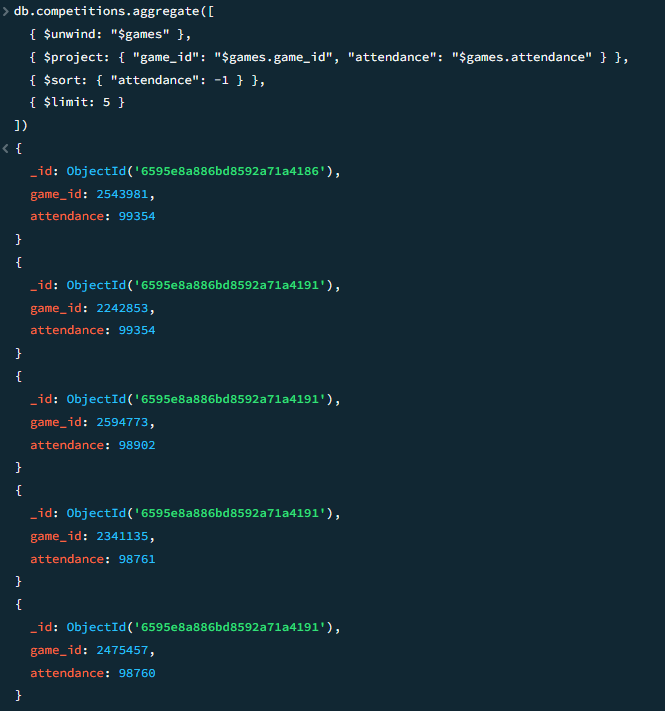
\includegraphics[scale=1]{Images/Queries/Competitions/most_followed_games/mfg.png}
    \caption{Most Followed Matches First Query Execution}
\end{figure}
The second query returns the most followed matches filtering by competition. It is inserted a placeholder "$<$competition\_id$>$" to search the preferred league. In the picture competition\_id is equal to CL (Champions League)
\begin{verbatim}
    db.competitions.aggregate([
        { $match: { "competition_id": "<competition_id>" } },
        { $unwind: "$games" },
        { $project: { "game_id": 
            "$games.game_id", "attendance": "$games.attendance", "competition_id": 1 } },
        { $sort: { "attendance": -1 } },
        { $limit: 5 }
      ])           
\end{verbatim}
\begin{figure}[htbp]
    \centering
    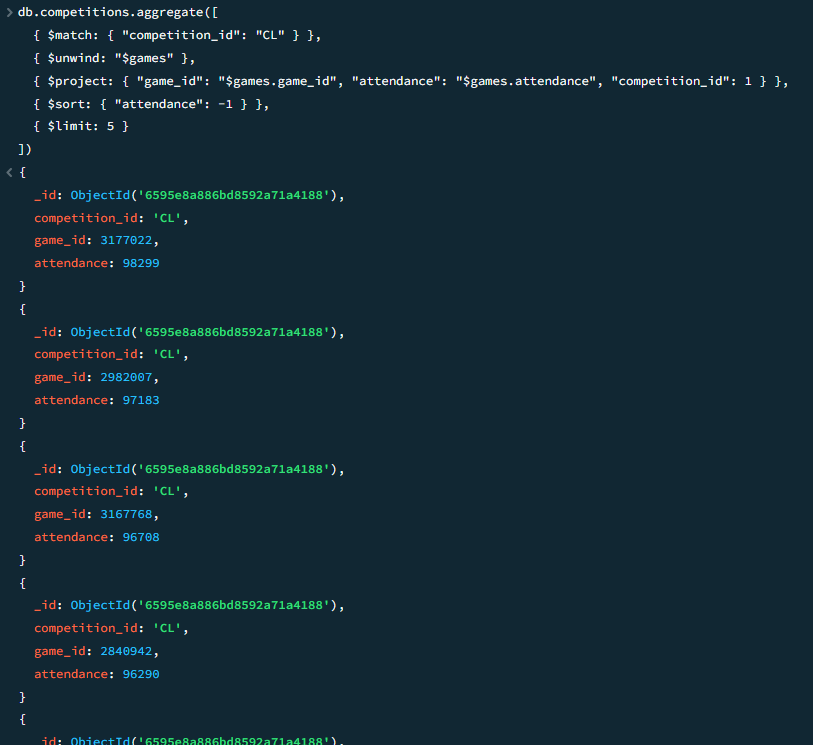
\includegraphics[scale=1]{Images/Queries/Competitions/most_followed_games/mfgcl.png}
    \caption{Most Followed Matches Second Query Execution}
\end{figure}

\subsection{Most goals scored by a single team}
These queries are designed to retrieve the games with the highest number of goals scored by a single team, with the second one specifically filtering for games within the "Champions League" competition. They unwind the games array, calculate the maximum goals scored in a game, sort the results by this maximum in descending order, and limit the output to the top 5 records.
\begin{verbatim}
  db.competitions.aggregate([
    { $unwind: "$games" },
    { $project: { game_id: "$games.game_id", maxGoals: { $max: ["$games.home_club_goals", "$games.away_club_goals"] } } },
    { $sort: { maxGoals: -1 } },
    { $limit: 5 }
  ])

  db.competitions.aggregate([
    { $match: { "competition_id": "CL" } },
    { $unwind: "$games" },
    { $project: { game_id: "$games.game_id", maxGoals: { $max: ["$games.home_club_goals", "$games.away_club_goals"] } } },
    { $sort: { maxGoals: -1 } },
    { $limit: 5 }
  ])
  
\end{verbatim}
\begin{figure}[htbp]
    \centering
    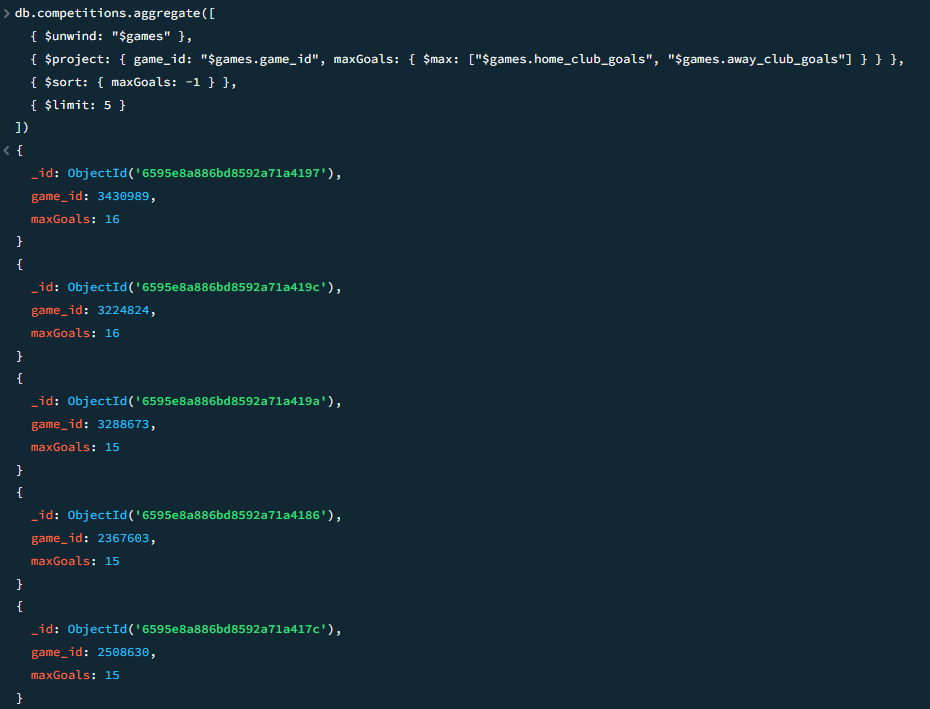
\includegraphics[scale=0.8]{Images/Queries/Competitions/most_goal_single_teams/mgst.png}
    \caption{Most Followed Matches First Query Execution}
\end{figure}
\begin{verbatim}
    db.competitions.aggregate([
        { $match: { "competition_id": "<competition_id>" } },
        { $unwind: "$games" },
        { $group: { _id: "$games.home_club_name", homeWins: 
            { $sum: { $cond: [{ $gt: 
                ["$games.home_club_goals", "$games.away_club_goals"] }, 1, 0] } } } },
        { $sort: { homeWins: -1 } },
        { $limit: 5 }
      ]) 
\end{verbatim}

\begin{figure}[htbp]
    \centering
    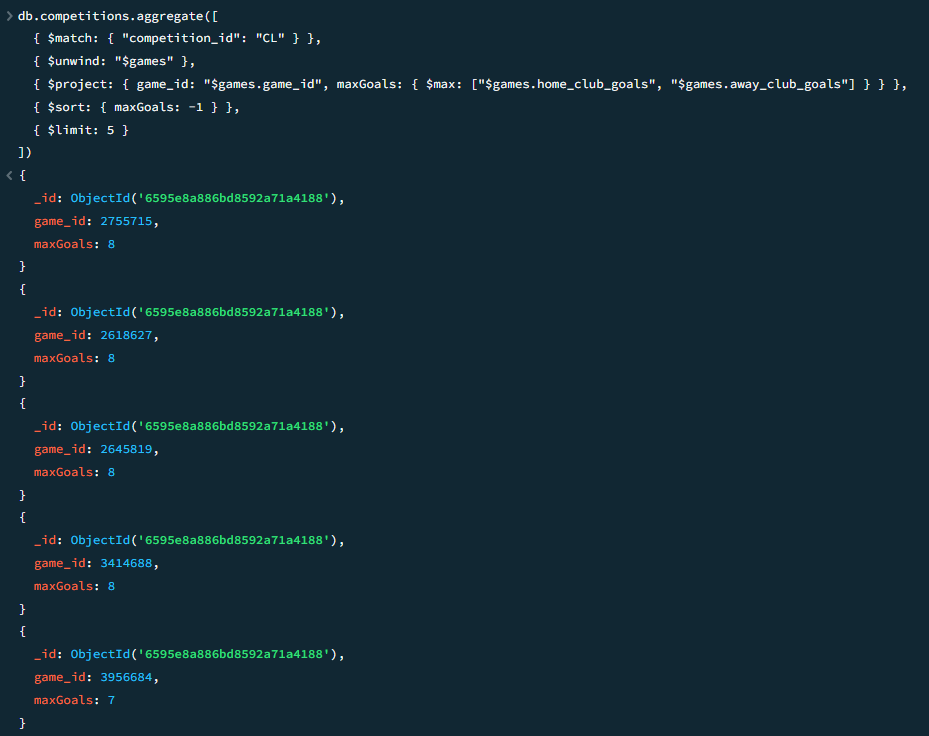
\includegraphics[scale=0.8]{Images/Queries/Competitions/most_goal_single_teams/mgstcl.png}
    \caption{Most Followed Matches Second Query Execution}
\end{figure}

\subsection{The most successful coaches}
This query shows the most important coaches ordered by win. This query was very difficult because the names of the coaches are present inside games, but in games there are 2 managers: one of the home club and one of the away club.\\
To exclude null values from the final result and not count unknown managers, you can modify the query by adding a condition to discard documents where the manager name is null before performing the final aggregation.The creation of the query followed these steps:
\begin{enumerate}
    \item \$unwind: Breaks down the array games.
    \item \$project: Creates fields representing home and away wins and manager names.
    \item \$group: Group at the collection level to create arrays with home and away manager wins.
    \item \$project: Concatenates arrays of home and away wins.
    \item \$unwind: Breaks down the concatenated array.
    \item \$match: Adds a filter to discard records where the manager name is null.
    \item \$group: Groups by manager name, summing wins and discarding null managers.
    \item \$sort: Sorts managers by total number of wins in a descending manner.
    \item \$match: This final step excludes documents with \_id null from the result set, removing unknown managers.
\end{enumerate}
\begin{verbatim}
    db.competitions.aggregate([
        { $unwind: "$games" },
        { $project: {
          homeManager: "$games.home_club_manager_name",
          awayManager: "$games.away_club_manager_name",
          homeWin: { $cond: { if: 
          { $gt: [ "$games.home_club_goals", "$games.away_club_goals" ] }, 
            then: 1, else: 0 } },
          awayWin: { $cond: { if: 
          { $gt: [ "$games.away_club_goals", "$games.home_club_goals" ] }, 
            then: 1, else: 0 } }
        }},
        { $group: {
          _id: null,
          homeManagerWins: { $push: { k: "$homeManager", v: "$homeWin" } },
          awayManagerWins: { $push: { k: "$awayManager", v: "$awayWin" } }
        }},
        { $project: {managerWins: 
            { $concatArrays: [ "$homeManagerWins", "$awayManagerWins" ] }
        }},
        { $unwind: "$managerWins" },
        { $match: { "managerWins.k": { $ne: null } } }, // esclude i manager non noti
        { $group: {
          _id: "$managerWins.k",
          totalWins: { $sum: "$managerWins.v" }
        }},
        { $sort: { totalWins: -1 } },
        { $match: { _id: { $ne: null } } } // esclude i risultati dove il nome del manager è null
      ])
      
\end{verbatim}
\begin{figure}[htbp]
    \centering
    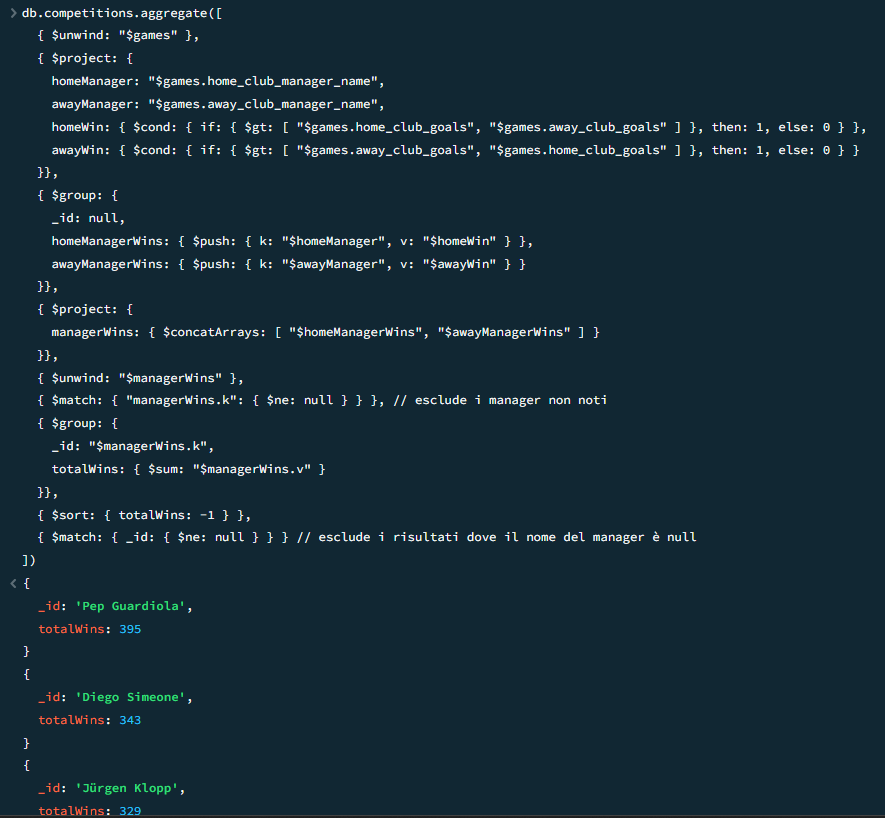
\includegraphics[scale=0.8]{Images/Queries/Competitions/most_succesful_coaches/msc.png}
    \caption{The most successful coaches Query Execution}
\end{figure}

\section{Clubs Collection}
\subsection{Clubs with more late goals}
The query runs through the 'clubs' collection, expands the 'games' array and its 'events' for each club, then filtering out events that are goals scored beyond the 80th minute. It then groups the results by 'club\_code' and counts the late goals for each club, sorting the clubs by the number of these goals.
\begin{verbatim}
    db.clubs.aggregate([
  { $unwind: "$games" },
  { $unwind: "$games.events" },
  { $match: { "games.events.type": "Goals", "games.events.minute": { $gt: 80 } } },
  { $group: { _id: "$club_code", lateGoals: { $sum: 1 } } },
  { $sort: { lateGoals: -1 } }
])
\end{verbatim}
\begin{figure}[htbp]
    \centering
    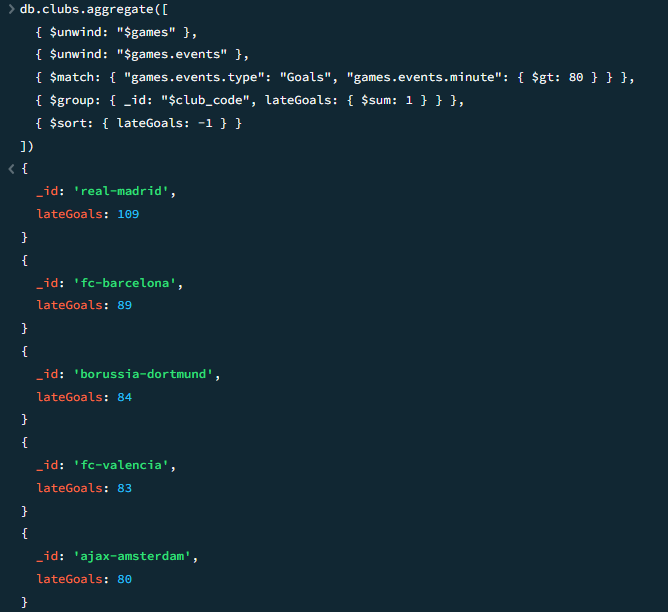
\includegraphics[scale=0.8]{Images/Queries/Clubs/late_goals_per_club/lgpc.png}
    \caption{The most successful coaches Query Execution}
\end{figure}
\subsection{Clubs with most foreign players}
The query selects all clubs and projects only the 'club\_code' and the 'foreigners\_percentage,' which is the percentage of foreign players in the team. It then sorts the clubs from highest to lowest percentage, to show which clubs have the largest proportion of foreign players in their roster.
\begin{verbatim}
    db.clubs.find({}, 
    {"club_code": 1, "foreigners_percentage":1}).sort(
        { foreigners_percentage: -1 }).limit(5)
\end{verbatim}

\begin{figure}[htbp]
    \centering
    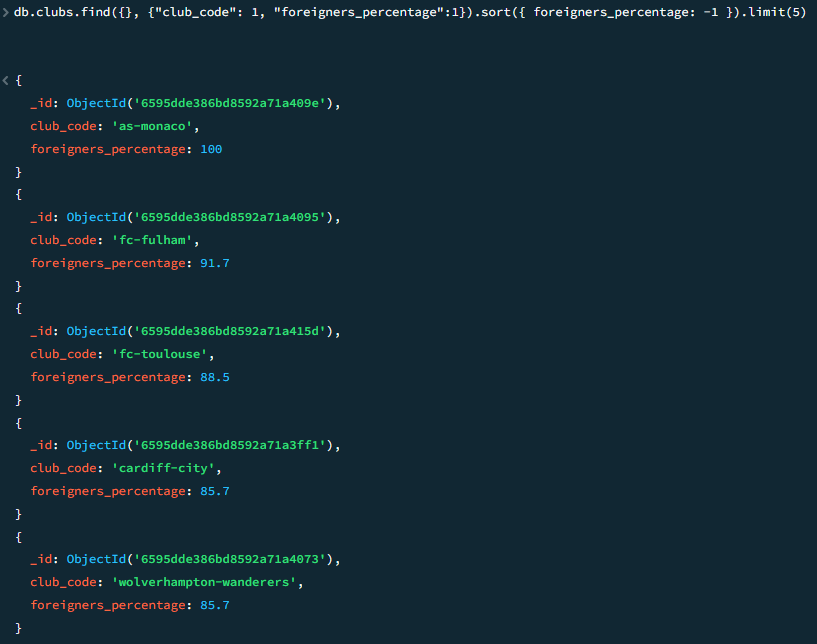
\includegraphics[scale=0.8]{Images/Queries/Clubs/Foreign_percentages/fp.png}
    \caption{Clubs with most foreign players Query Execution}
\end{figure}

\subsection{Clubs with more wins at home}
This query identifies clubs that have scored the most goals in home games. After expanding the array games, it filters for games played at home and sums the goals scored in these games. Finally, it sorts the clubs by the total number of goals scored at home.
\begin{verbatim}
    db.clubs.aggregate([
  { $unwind: "$games" },
  { $match: { "games.hosting": "H" } },
  { $group: { _id: "$club_code", homeWins: 
    { $sum: { $cond: [{ $eq: ["$games.is_win", 1] }, 1, 0] } } } },
  { $sort: { homeWins: -1 } }
])
\end{verbatim}
\begin{figure}[htbp]
    \centering
    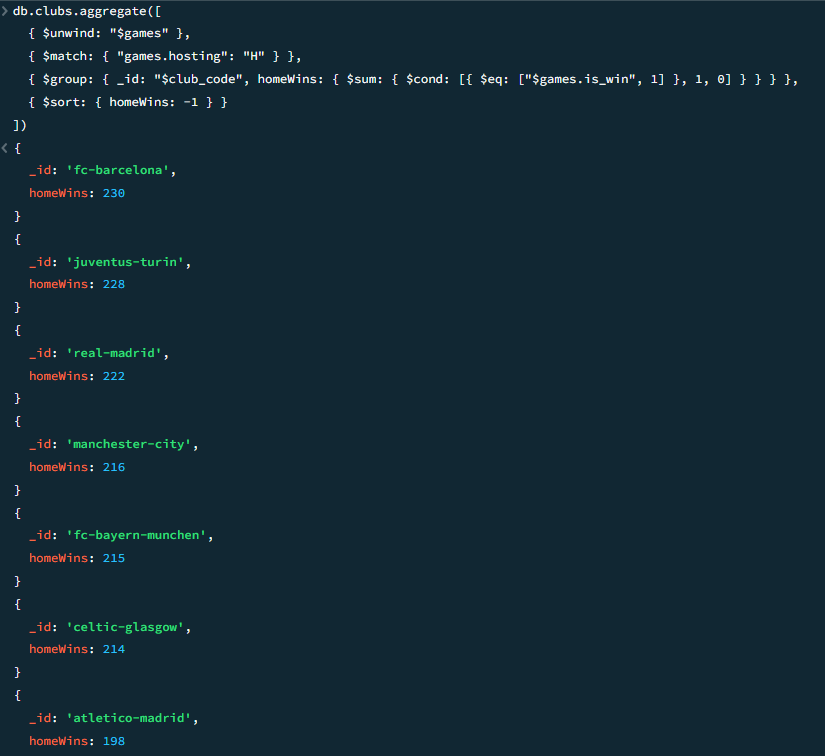
\includegraphics[scale=0.8]{Images/Queries/Clubs/more_wins_at_home/mwat.png}
    \caption{Clubs with more wins at home Query Execution}
\end{figure}

%-------------------------------------------------------------------------
%	APPENDICES
%-------------------------------------------------------------------------

\cleardoublepage
\addtocontents{toc}{\vspace{2em}} % Add a gap in the Contents, for aesthetics
\appendix
\chapter{Appendix A}
If you need to include an appendix to support the research in your thesis, you can place it at the end of the manuscript.
An appendix contains supplementary material (figures, tables, data, codes, mathematical proofs, surveys, \dots)
which supplement the main results contained in the previous chapters.


% LIST OF FIGURES
\listoffigures

% LIST OF TABLES
\listoftables

\cleardoublepage

\end{document}
